\documentclass{article}

\usepackage{neurips_2026}

\usepackage[utf8]{inputenc} % allow utf-8 input
\usepackage[T1]{fontenc}    % use 8-bit T1 fonts
\usepackage{hyperref}       % hyperlinks
\usepackage{url}            % simple URL typesetting
\usepackage{booktabs}       % professional-quality tables
\usepackage{amsfonts}       % blackboard math symbols
\usepackage{nicefrac}       % compact symbols for 1/2, etc.
\usepackage{microtype}      % microtypography
\usepackage{xcolor}         % colors

\usepackage{multirow}
\usepackage{amssymb}
\usepackage{graphicx}
\usepackage{natbib}
\usepackage{doi}
\usepackage{amsmath}
\usepackage{physics}
\usepackage{wrapfig}
\usepackage{bm}
\usepackage{algorithm,algpseudocode}
\usepackage{forest}
\usepackage{tcolorbox}
\usepackage{tikz-cd}
\usetikzlibrary{calc}
\usepackage{enumitem}

\usepackage{amsthm}

\newtheorem{theorem}{Theorem}
\newtheorem{lemma}{Lemma}
\newtheorem{proposition}{Proposition}
\newtheorem{corollary}{Corollary}

\theoremstyle{definition}
\newtheorem{definition}{Definition}
\newtheorem{assumption}{Assumption}

\theoremstyle{remark}
\newtheorem{remark}{Remark}
\newtheorem{example}{Example}

% Blackboard bold sets
\newcommand{\R}{\mathbb{R}}
\newcommand{\N}{\mathbb{N}}
\newcommand{\Z}{\mathbb{Z}}
\newcommand{\Q}{\mathbb{Q}}
\newcommand{\C}{\mathbb{C}}

% Labels
\newcommand{\alg}{\mathrm{alg}}
\newcommand{\meta}{\mathrm{meta}}
\newcommand{\fix}{\mathrm{fix}}

% Probability
\newcommand{\Prb}{\mathbb{P}}
\newcommand{\E}{\mathbb{E}}
\DeclareMathOperator{\Var}{Var}
\DeclareMathOperator{\Cov}{Cov}

% Operators
\DeclareMathOperator{\diag}{diag}
\DeclareMathOperator{\supp}{supp}

\newcommand{\argmax}{\operatorname*{arg\,max}}
\newcommand{\argmin}{\operatorname*{arg\,min}}
\newcommand{\ind}{\mathbf{1}}

% Inner product
\newcommand{\inner}[2]{\left\langle #1, #2 \right\rangle}

% Calligraphic sets
\newcommand{\cA}{\mathcal{A}}
\newcommand{\cS}{\mathcal{S}}
\newcommand{\cT}{\mathcal{T}}
\newcommand{\cF}{\mathcal{F}}
\newcommand{\cE}{\mathcal{E}}

% RL notation
\newcommand{\SSS}{\mathcal{S}}
\newcommand{\AAA}{\mathcal{A}}
\newcommand{\PP}{\mathcal{P}}
\newcommand{\RRR}{\mathcal{R}}
\newcommand{\gammaRL}{\gamma}

% Confidence bounds
\newcommand{\olQ}{\overline{Q}}
\newcommand{\ulQ}{\underline{Q}}
\newcommand{\olV}{\overline{V}}
\newcommand{\ulV}{\underline{V}}

% Misc
\newcommand{\eps}{\varepsilon}
\newcommand{\dt}{\mathrm{d}t}
\newcommand{\given}{\,\bigl\vert\,}

% Fractions
\newcommand{\half}{\tfrac12}
\newcommand{\thalf}{\tfrac32}

% Notes
\newcommand{\note}[1]{\paragraph{Note.} #1}

\theoremstyle{remark}
\newtheorem{conjecture}[theorem]{Conjecture}


\title{LinUCB Is (Almost) All You Need:\\ A Regime Analysis of LLM Warm-Starts in Contextual Bandits}


\author{%
  David S.~Hippocampus\thanks{Use footnote for providing further information
    about author (webpage, alternative address)---\emph{not} for acknowledging
    funding agencies.} \\
  Department of Computer Science\\
  Cranberry-Lemon University\\
  Pittsburgh, PA 15213 \\
  \texttt{hippo@cs.cranberry-lemon.edu} \\
}


\begin{document}
\maketitle
\begin{abstract}
A recent line of work reports striking ``reward multiplication'': combining a
frozen LLM policy with an adaptive contextual bandit dominates either component,
sometimes by an order of magnitude. We argue this is a \emph{regime indicator},
not a generic phenomenon---``cold-start LinUCB is (almost) all you need.''
We isolate three structural axes---effective dimension versus horizon,
\textbf{feature coherence}, and \textbf{action-gap structure}---and prove a
``LinUCB-suffices'' bound along each. Saturating axis~A or~B alone certifies
that no warm-start can improve cold-start LinUCB by more than a constant
factor; axis~C provides a gap-dependent save when the effective dimension is
moderate. The three-way separation behind the multiplication story lives where
axes A and B jointly deviate; a regret-balancing analysis sharpens this to a
phase transition at $r\asymp\sqrt T/\log T$. Four pre-runtime diagnostics
classify any instance into one of four regimes before any algorithm runs;
across every configuration we test, they correctly predict the order of
magnitude of the warm-start lift.
\end{abstract}


\section{Introduction}
\label{sec:intro}

Sequential decision making studies how an agent adapts to an unknown
environment through repeated interaction \cite{zhu2022largeaction,zhu2022contextual},
with applications in recommendation \cite{li2010contextual,agarwal2016making},
healthcare \cite{tewari2017ads,svensson2023sequential}, and dialogue
\cite{li2016deep}. Large pretrained language models supply strong prior
knowledge that can guide early decisions
\cite{brown2020language,ouyang2022training,achiam2023gpt,
alamdari2024jumpstarting,abbasiyadkori2024believe}.

A striking observation is that combining a frozen LLM with an adaptive
contextual bandit appears to strictly dominate either component, sometimes by
orders of magnitude \cite{chen2024llmdecision,huangcontextual}. This
\emph{reward multiplication} phenomenon is empirically robust and mechanistically
intuitive. Yet bandit warm-starting \cite{bastani2021mostly,zhang2019warm} and
confidence-gated model selection
\cite{auer2002nonstochastic,agarwal2017corralling,pacchiano2020model} are not
new objects, and the older literature does \emph{not} report comparable
multipliers. We take that discrepancy seriously and ask the dual question:
\emph{when is plain cold-start LinUCB enough?} If ``almost always,''
multiplication is a regime indicator, and the question shifts from ``how do
we get it?'' to ``what structural property of the dataset enables it, and can
we predict it in advance?''

We claim that cold-starting LinUCB is competitive with any warm-started
variant up to a constant factor on \emph{any} instance saturating one of
three structural axes; in our experiments, this covers every configuration
except one. Multiplicative gain requires joint failure of
\textbf{(A)~ambient versus effective dimension} and \textbf{(B)~feature
coherence}, with \textbf{(C)~action-gap structure} acting as a third
gap-dependent save when the effective dimension is moderate. The three-way
separation underlying the original mechanism story
(\cite{chen2024llmdecision}, restated as Proposition~\ref{prop:three-way})
lives at the corner where axes A and B both fail; axis~C is saturated in that
construction (uniform gap $1$) yet warm-starting still helps because the
gap-dependent bound is vacuous when $r=T$. The axes are sufficient conditions
in priority order: axis~A is the dimensional phase transition
$r\!\asymp\!\sqrt T/\log T$ (primary); axis~B saturates whenever features
have positive coherence (typical of pretrained embeddings); axis~C saves
only when $r$ is moderate. We render this as a hierarchical decision tree
(Figure~\ref{fig:tree}); reaching the bottom ``warm-start-essential'' leaf
requires axes A and B both to fail and axis~C to fail or be vacuous due to
large $r$. Four dataset-level statistics classify any instance into one of
four regimes before any algorithm runs, correctly predicting whether
warm-starting helps on every configuration tested
(Section~\ref{sec:experiments})---including previously unexplained negative
lifts and the multi-fold gains uniquely flagged as warm-start-essential. A
comprehensive related-works discussion is in Appendix~\ref{sec:related}.

\paragraph{Contributions.}
\begin{itemize}[itemsep=1pt, topsep=1pt, leftmargin=*]
\item \textbf{Regime-indicator framework.} A ``LinUCB-suffices'' lemma along
each axis (Lemmas~\ref{lem:low-effective-dim}, \ref{lem:coherent-suffices},
\ref{lem:gap-suffices}) paired with sharp-threshold extensions in the
complementary direction (Lemmas~\ref{lem:sparse-reward}, \ref{lem:pseudo-orth},
\ref{lem:vanishing-gap}, in appendix). The original separation
\cite{chen2024llmdecision} (Proposition~\ref{prop:three-way}) is the joint
corner (Corollary~\ref{cor:joint-corner}).
\item \textbf{Confidence-gated meta-algorithm with regime-aware guarantees.}
Theorem~\ref{thm:warm-start-regret} gives shrinkage factor
$\Psi(\tau,\nu,T)\!\le\!\sqrt{\lambda/(\lambda+\nu\tau)}$, bounded strictly
below $1$ horizon-independently \emph{only} when all three axes deviate. The
phase transition $r\!\asymp\!\sqrt T/\log T$ (Theorem~\ref{thm:avg-mult})
is the formal version of axis~A.
\item \textbf{Pre-runtime diagnostics, empirically validated.} Four measurable
statistics classify each instance \emph{before} any decision-making algorithm
runs and correctly predict sign and order of magnitude of the warm-start lift
on every configuration tested---including negative lifts not predicted by
previous treatments.
\end{itemize}


\section{Preliminaries}
\label{sec:preliminaries}

We work in a standard linear contextual bandit setting
\cite{zhu2022largeaction,zhu2022contextual}. At each round $t=1,\dots,T$, the
learner observes a finite action set $\mathcal A_t$ where each
$a\!\in\!\mathcal A_t$ has a feature vector $x_{t,a}\!\in\!\mathbb R^d$ with
$\|x_{t,a}\|_2\le L$, selects $A_t\!\in\!\mathcal A_t$, and observes reward
$r_t = \langle\theta^\star,x_{t,A_t}\rangle + \eta_t$, where
$\theta^\star\!\in\!\mathbb R^d$ is unknown with $\|\theta^\star\|_2\le S$ and
$\eta_t$ is conditionally mean-zero $\sigma$-sub-Gaussian. Write
$\mu_t(a)=\langle\theta^\star,x_{t,a}\rangle$ and
$a_t^\star\!\in\!\arg\max_a\mu_t(a)$. The cumulative pseudo-regret of a policy
$\pi$ is $R_T(\pi)=\sum_t(\mu_t(a_t^\star)-\mu_t(\pi_t))$.

The learner has access to two qualitatively different decision rules:
\textbf{(1)} a \emph{frozen policy} induced by some estimator
$\widehat\theta\!\in\!\mathbb R^d$ with associated design matrix
$V\!\succ\!0$, never updated online; \textbf{(2)} an \emph{adaptive bandit
algorithm} (LinUCB), which maintains
$V_t=\lambda I + \sum_{s<t}x_{s,A_s}x_{s,A_s}^\top$,
$b_t=\sum_{s<t}r_s x_{s,A_s}$, $\widehat\theta_t=V_t^{-1}b_t$, and selects
$A_t\!\in\!\arg\max_a\langle\widehat\theta_t,x_{t,a}\rangle+\beta_t\|x_{t,a}\|_{V_t^{-1}}$.
The frozen policy may be an LLM, a regression head on pretrained features, or
any other offline-trained predictor. The structural asymmetry: the frozen
policy may be good initially but cannot improve, while the adaptive algorithm
may be weak initially but improves with data. \emph{When, if ever, is the
frozen policy strictly necessary?}

\paragraph{Cold-started and warm-started LinUCB.}
\emph{Cold-started LinUCB} is rule (2) with $V_1=\lambda I_d$ and $b_1=0$.
\emph{Warm-started LinUCB} replaces these with
\begin{equation}
\label{eq:warm-start-def}
V_1 = \lambda I_d + M, \qquad b_1 = c,
\end{equation}
for symmetric PSD $M\!\succeq\!0$ and offset $c\!\in\!\mathbb R^d$. The
canonical $(M,c)$ is the empirical Gram and response sum from $N$ rollouts of
a fixed logging policy: $M=\sum_s x_sx_s^\top$, $c=\sum_s r_s x_s$. The
rollouts may come from offline data at $t=1$, or from an online meta-algorithm
that routes early decisions to a frozen expert. Decision-tree
Figure~\ref{fig:tree} is a property of the \emph{instance}, not of $(M,c)$,
and governs whether \emph{any} $(M,c)$ can deliver more than a constant-factor
regret reduction. ``No warm-start can improve cold-started LinUCB by more
than a constant factor'' means there exists a universal $C$ such that
$R_T^{\mathrm{warm}}/R_T^{\mathrm{cold}}\le C$ in the leading order in $T$
for every $(M,c)$ obtained from $N=O(T)$ rollouts; ``warm-starting is
essential'' means $R_T^{\mathrm{cold}}/R_T^{\mathrm{warm}}\to\infty$ for some
$(M,c)$. Figure~\ref{fig:tree} characterizes where the latter is possible:
only at the bottom red leaf.


\section{Main Results}
\label{sec:main-results}

Section~\ref{sec:axes} isolates three structural axes that govern whether
warm-starting can produce a multiplicative gain over cold-start LinUCB, and
proves a paired ``LinUCB-suffices'' lemma along each.
Section~\ref{sec:diagnostics} introduces the four pre-runtime diagnostics that
classify any instance into a regime.
Section~\ref{sec:master-multiple} introduces the confidence-gated
meta-algorithm, states the warm-started regret bound, and translates it into
an average-reward multiplication theorem with a dimensional phase transition.
All proofs are deferred to Appendix~\ref{app:proofs}.

\subsection{Three Structural Axes for Reward Multiplication}
\label{sec:axes}

The construction in \cite{chen2024llmdecision} (Proposition~\ref{prop:three-way}
below) has \emph{exactly} three structural ingredients---strict feature
orthogonality, ambient dimension matching the horizon, and a fixed gap hidden
inside an optimism trap---and the linear-regret behaviour collapses if
\emph{any one} is removed. Conversely, every $\widetilde O(\sqrt{rT})$ upper
bound for cold-start LinUCB \cite{abbasi2011improved,chu2011contextual,
dani2008stochastic,lattimore2020bandit} is sub-optimal only when (A)~the
effective dimension $r$ is comparable to $T$, (B)~features are pairwise
orthogonal so the determinant ratio cannot be amortized across arms, or
(C)~the action gap vanishes so the $\sqrt T$-rate cannot be sharpened to
$\log T$. Reaching the bottom red leaf of Figure~\ref{fig:tree} requires
\emph{simultaneous} failure on all three.

\begin{figure}[t]
\centering
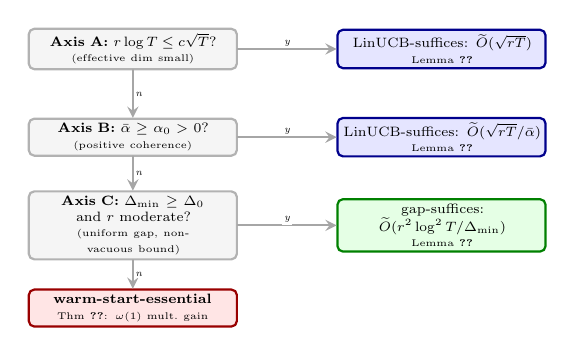
\begin{tikzpicture}[
    scale=0.7, every node/.style={transform shape},
    >=stealth, line cap=round, line join=round,
    decision/.style={rectangle, rounded corners=2pt, draw=gray!60, thick,
      fill=gray!8, align=center, inner sep=2.5pt, text width=3.6cm, font=\scriptsize},
    safeleaf/.style={rectangle, rounded corners=2pt, thick, align=center,
      inner sep=2.5pt, text width=3.6cm, font=\scriptsize},
    blueleaf/.style={safeleaf, draw=blue!55!black, fill=blue!10},
    greenleaf/.style={safeleaf, draw=green!50!black, fill=green!10},
    redleaf/.style={safeleaf, draw=red!60!black, fill=red!10},
    edgeline/.style={->, draw=gray!70, thick},
    yestag/.style={font=\tiny\itshape, inner sep=1pt, fill=white},
    notag/.style={font=\tiny\itshape, inner sep=1pt, fill=white}
]
  \node[decision] (B) at (0,0)
    {\textbf{Axis A:} $r\log T\!\le\! c\sqrt T$? \\ \tiny (effective dim small)};
  \node[decision] (A) at (0,-1.6)
    {\textbf{Axis B:} $\bar\alpha\!\ge\!\alpha_0\!>\!0$? \\ \tiny (positive coherence)};
  \node[decision] (C) at (0,-3.2)
    {\textbf{Axis C:} $\Delta_{\min}\!\ge\!\Delta_0$ and $r$ moderate? \\ \tiny (uniform gap, non-vacuous bound)};
  \node[redleaf] (essential) at (0,-4.7)
    {\textbf{warm-start-essential} \\ \tiny Thm~\ref{thm:warm-start-regret}: $\omega(1)$ mult.\ gain};
  \node[blueleaf] (Bleaf) at (5.6,0)
    {LinUCB-suffices: $\widetilde O(\sqrt{rT})$ \\ \tiny Lemma~\ref{lem:low-effective-dim}};
  \node[blueleaf] (Aleaf) at (5.6,-1.6)
    {LinUCB-suffices: $\widetilde O(\sqrt{rT}/\bar\alpha)$ \\ \tiny Lemma~\ref{lem:coherent-suffices}};
  \node[greenleaf] (Cleaf) at (5.6,-3.2)
    {gap-suffices: $\widetilde O(r^2\log^2 T/\Delta_{\min})$ \\ \tiny Lemma~\ref{lem:gap-suffices}};
  \draw[edgeline] (B.east)  -- node[yestag, above]{y} (Bleaf.west);
  \draw[edgeline] (B.south) -- node[notag,  right]{n}  (A.north);
  \draw[edgeline] (A.east)  -- node[yestag, above]{y} (Aleaf.west);
  \draw[edgeline] (A.south) -- node[notag,  right]{n}  (C.north);
  \draw[edgeline] (C.east)  -- node[yestag, above]{y} (Cleaf.west);
  \draw[edgeline] (C.south) -- node[notag,  right]{n}  (essential.north);
\end{tikzpicture}
\caption{Decision tree for LinUCB-suffices vs.\ warm-start-essential. Axis~A
is primary (the phase transition $r\asymp\sqrt T/\log T$); axes~B and~C are
secondary rescuers. Reaching the red leaf requires \emph{all three} conditions
to fail simultaneously (Corollary~\ref{cor:joint-corner}).}
\label{fig:tree}
\end{figure}

\paragraph{The classical worst case.}
\cite{chen2024llmdecision} use horizon $n$, single reward direction $g=e_1$,
and $n$ orthogonal ``bad'' directions $b_t=Le_{t+1}$ ($L>1$); optimism induced
by $\|b_t\|_2\!=\!L\!>\!1$ in $V_0\!=\!\lambda I$ forces cold-start LinUCB to
pull $b_t$ at every round.

\begin{proposition}[Three-way separation; \cite{chen2024llmdecision}]
\label{prop:three-way}
Fix horizon $n\!\ge\!1$, $L\!>\!1$, $\lambda\!>\!0$. There exist a dimension
$d\!\ge\!n+1$, parameter $\theta^\star\!\in\!\mathbb R^d$, and two-action sets
$\{\mathcal A_t\}_{t=1}^n$ such that, for any sub-Gaussian noise model:
(1) some constant policy $\pi_{\mathrm{const}}$ has cumulative pseudo-regret
exactly $n$; (2) cold-start LinUCB also incurs regret $n$ (selecting the same
action as $\pi_{\mathrm{const}}$ each round); (3) for any $m$ sufficiently
large, LinUCB warm-started with the design matrix that $\pi_{\mathrm{const}}$
generates from $mn$ offline rollouts incurs $O(1)$ regret w.p.\ $\ge 1-\delta$.
\end{proposition}

The construction is fragile in three specific ways, each individually
\emph{necessary}: \textbf{(A)} ambient dimension $d\!\ge\!n+1$;
\textbf{(B)} strict orthogonality (otherwise pulling $b_s$ leaks information
about $b_t$ or $g$); \textbf{(C)} the optimism trap, which is uninterrupted
by an action gap. We extend along each axis below; full proofs and
sharp-threshold negative companions
(Lemmas~\ref{lem:sparse-reward}, \ref{lem:pseudo-orth},
\ref{lem:vanishing-gap}) are in Appendix~\ref{app:proofs}.

\paragraph{Axis A: Ambient versus effective dimension.}

\begin{lemma}[Saturated coverage]
\label{lem:low-effective-dim}
Let $r$ denote the effective dimension of the reward-relevant subspace. If
$r\log T\le c\sqrt T$ for any $c>0$, then cold-started LinUCB attains
$R_T^{\mathrm{cold}}=\widetilde O(\sqrt{rT})$, and the same rate holds for
any warm-started LinUCB$(M,c)$. Cold-start matches warm-start up to a
constant factor.
\end{lemma}

In cumulative regret, warm-starting can still shave a constant factor; in
average-reward terms, that constant-factor reduction does not translate into
an $\Omega(1)$-factor gain. The lemma's complementary negative result---a
$\Omega(\sqrt{d/r})$ multiplicative gain when $r\!=\!T$---is
Lemma~\ref{lem:sparse-reward}.

\paragraph{Axis B: Feature coherence.}

\begin{lemma}[Coherent features]
\label{lem:coherent-suffices}
Suppose features satisfy a uniform positive lower-coherence condition: there
exists $\bar\alpha\in(0,1]$ with
$\langle x_{t,a},x_{t,a'}\rangle \ge \bar\alpha\,\|x_{t,a}\|\|x_{t,a'}\|$
for all $t$ and all $a,a'\in\mathcal A_t$. Then cold-started LinUCB satisfies
$R_T^{\mathrm{cold}}=\widetilde O(\sqrt{rT}/\bar\alpha)$, and any
warm-started LinUCB$(M,c)$ with $N=O(T)$ rollouts attains the same order. The
linear-regret instance of Proposition~\ref{prop:three-way} \emph{cannot exist}
on any feature distribution with $\bar\alpha$ bounded strictly above $0$.
\end{lemma}

The proof shows that positive coherence forces every off-arm pull to contract
LinUCB's confidence width on the optimal action by a multiplicative
$1-\bar\alpha^2\rho_t$ factor; the standard elliptical-potential argument
\cite{abbasi2011improved} then gives a $\sqrt T$-rate. The hypothesis is
demanding (worst-case coherence over all pairs), and a weaker average-case
condition likely suffices empirically; we use a robust median-based proxy in
Section~\ref{sec:diagnostics}, and the gap between the empirical proxy and
the worst-case sufficient condition is discussed in
Appendix~\ref{app:diagnostics}. The threshold is sharp at $\bar\alpha=0$:
Proposition~\ref{prop:three-way} achieves linear regret precisely because its
features are exactly orthogonal. Extending to
$\bar\mu$-pseudo-orthogonality at the sharp scale $\bar\mu\asymp 1/\sqrt n$
is Lemma~\ref{lem:pseudo-orth}.

\paragraph{Axis C: Action-gap structure.}

\begin{lemma}[Uniform gap]
\label{lem:gap-suffices}
Suppose there exists $\Delta_{\min}>0$ with
$\mu_t(a_t^\star)-\mu_t(a)\ge\Delta_{\min}$ for every $t$ and every
$a\in\mathcal A_t\setminus\{a_t^\star\}$. Then $R_T^{\mathrm{cold}}\le
Cr\beta_T^2\log T/\Delta_{\min}=\widetilde O(r^2\log^2 T/\Delta_{\min})$, and
any warm-started LinUCB$(M,c)$ with $N=O(T)$ rollouts attains the same order.
The bound is non-vacuous only when $r^2\log^2 T/\Delta_{\min}=o(T)$; in
particular, when $r\asymp T$, axis~C provides no save.
\end{lemma}

\paragraph{The joint corner condition.}
Each lemma controls one mechanism; linear-regret behaviour requires
\emph{(i)} simultaneous failure on axes A and B, \emph{or}, when axis~A fails
alone, additional failure on axis~C.

\begin{corollary}[Joint corner]
\label{cor:joint-corner}
For the meta-algorithm of Section~\ref{sec:master-multiple} to provide a
multiplicative regret reduction strictly more than a constant factor over
cold-start LinUCB, the instance must lie outside every LinUCB-suffices
regime: $r\log T\!\gg\!\sqrt T$ \emph{(A)}, $\bar\alpha$ below the coherence
threshold of Lemma~\ref{lem:coherent-suffices} \emph{(B)}, and either
$\Delta_{\min}\!\to\!0$ or $r$ large enough that the gap-dependent bound
exceeds the gap-independent $\sqrt{rT}$ bound \emph{(C)}.
\end{corollary}

In Proposition~\ref{prop:three-way}, the uniform gap is $1$ but $r=n=T$, so
the gap-dependent bound $\widetilde O(r^2\log^2 T/\Delta_{\min})=\widetilde O(T^2)$
is vacuous and axis~C provides no save---consistent with the corollary.

\subsection{Pre-Runtime Regime Diagnostics}
\label{sec:diagnostics}

Each axis is empirically measurable from an offline sample of contexts
\emph{before} running any algorithm. We use three instance-level statistics
plus one LLM-conditional refinement (formal definitions and concentration
guarantees: Appendix~\ref{app:diagnostics}):
\textbf{(A)} effective rank
$\widehat r := \mathrm{tr}(\widehat\Sigma)/\|\widehat\Sigma\|_{\mathrm{op}}$
(LinUCB-suffices when $\widehat r\log T/\sqrt T < c_0$; we use $c_0=0.1$);
\textbf{(B)} coherence $\widehat{\bar\alpha}$, the median over actions of
the minimum pairwise cosine similarity (LinUCB-suffices when
$\widehat{\bar\alpha}\ge\alpha_0$; we use $\alpha_0=0.1$);
\textbf{(C)} oracle gap distribution from a ridge-fit linear model trained on
labeled (context, action, reward) tuples (heavy left tail at zero indicates
Lemma~\ref{lem:vanishing-gap}); and
\textbf{(A$+$C)} subspace mismatch, the maximum principal angle between the
rank-$\widehat r$ subspaces of $V^{(i^\star)}$ and the online context
covariance.
The four diagnostics induce a pre-runtime classifier
$\mathsf{Regime}(\mathcal D)\!\in\!\{\textsf{LinUCB-suffices},
\textsf{gap-suffices},\textsf{warm-start-essential},\textsf{ambiguous}\}$
that identifies which leaf an instance reaches without inspecting the LLM.
The deployment decision is purely instance-level; whether a deployed
meta-algorithm \emph{realizes} its theoretical multiplier is a separate
question, governed by three LLM-quality conditions Q1--Q3
(Appendix~\ref{app:diagnostics}). Section~\ref{sec:experiments} reports the
diagnostics on each configuration alongside the realized lift; the regime
predictions match every sign and order of magnitude observed.

\subsection{Confidence-Gated Meta-Algorithm and Warm-Start Regret}
\label{sec:master-multiple}

The algorithm presented here is the deployment-time tool for instances at
the warm-start-essential leaf of Figure~\ref{fig:tree}. On every other leaf,
cold-start LinUCB already attains the optimal-up-to-constants rate and the
meta-algorithm is, at best, a constant-factor improvement.

We assume access to $m$ frozen policy estimators
$\{(\widehat\theta_i,V^{(i)})\}_{i=1}^m$ (e.g., LLM-induced linear predictors)
alongside an online LinUCB learner. At each round, each frozen expert
$i\!\in\![m]$ proposes $a_t^{(i)}\!\in\!\arg\max_a\langle\widehat\theta_i,x_{t,a}\rangle$
with confidence
$u_t^{(i)}\!:=\!\|x_{t,a_t^{(i)}}\|_{(V^{(i)})^{-1}}$; LinUCB proposes
$a_t^{(0)}$ with $u_t^{(0)}\!:=\!\|x_{t,a_t^{(0)}}\|_{V_t^{-1}}$. The
deterministic rule routes to the candidate with smallest uncertainty, with
an optional one-way handover to LinUCB once a $K$-round LCB-vs-UCB criterion
fires. Unlike CORRAL-style randomized masters \cite{agarwal2017corralling},
the deterministic rule lets the LinUCB sufficient statistics $(V_t,b_t)$ be
updated deterministically on every round, including expert-routed rounds---
the geometric mechanism behind the shrinkage factor below.\footnote{The
contextual-bandit master of \cite{chen2024llmdecision} uses a randomized
CORRAL-style update for routing but, like our deterministic master, also
passes every observed reward into the bandit base-learner state; the
distinction we exploit here is the deterministic per-round geometric routing,
not whether observations reach the base learner.} Pseudocode and walkthrough
are in Appendix~\ref{app:meta-algorithm}.

\paragraph{Setup and assumptions.}
The meta-algorithm makes a binary choice each round: route to LinUCB
($I_t=0$) or to a frozen expert ($I_t\!\in\![m]$). Let
$\mathcal T_{\mathrm{exp}}\!:=\!\{t:I_t\!\ne\!0\}$,
$\mathcal T_{\mathrm{lin}}\!:=\!\{t:I_t\!=\!0\}$,
$\tau\!:=\!|\mathcal T_{\mathrm{exp}}|$,
$\Delta_t^{(I_t)}\!:=\!\mu_t(a_t^\star)-\mu_t(a_t^{(I_t)})$. Conditional on
the instance being warm-start-essential, we impose:
\textbf{(A) uniform early quality:} $\Delta_t^{(I_t)}\!\le\!\varepsilon_0$
for every $t\!\in\!\mathcal T_{\mathrm{exp}}$;
\textbf{(B) reward-relevant warm-start coverage:} there is an $r$-dim
projector $P$ with $\theta^\star,x_{t,a}\!\in\!\mathrm{Im}(P)$ and
$\sum_{t\in\mathcal T_{\mathrm{exp}}}x_{t,A_t}x_{t,A_t}^\top\!\succeq\!\nu\tau P$
for some $\nu>0$.

\begin{theorem}[Warm-started cumulative regret]
\label{thm:warm-start-regret}
Assume rewards follow the linear model with $\sigma$-sub-Gaussian noise and
$\|x_{t,a}\|_2\!\le\!L$, and that Assumptions A and B hold. With probability
at least $1-\delta$, for any realization of $\tau$,
\begin{equation}
\label{eq:warm-meta-regret}
R_T^{\mathrm{meta}}
\;\le\;
\tau\varepsilon_0
+ C\beta_T\sqrt{r(T-\tau)\log\!\bigl(1+\tfrac{L^2(T-\tau)}{\lambda+\nu\tau}\bigr)},
\end{equation}
compared to the cold-started bound
\begin{equation}
\label{eq:cold-regret}
R_T^{\mathrm{cold}}\;\le\; C\beta_T\sqrt{rT\log(1+L^2T/\lambda)}.
\end{equation}
Equivalently, the post-handover term is a multiplicative shrinkage of the
cold-start bound:
\begin{equation}
\label{eq:psi-shrinkage}
R_T^{\mathrm{meta}}-\tau\varepsilon_0\;\le\;\Psi(\tau,\nu,T)\cdot R_T^{\mathrm{cold}},
\quad
\Psi(\tau,\nu,T)
=\sqrt{\tfrac{T-\tau}{T}}\cdot
\sqrt{\tfrac{\log(1+L^2(T-\tau)/(\lambda+\nu\tau))}{\log(1+L^2T/\lambda)}}.
\end{equation}
When $\nu\tau\gg\lambda$ and $\tau=o(T)$ (so that
$T-\tau=\Theta(T)$ and the prefactor $\sqrt{(T-\tau)/T}\to 1$), the
asymptotic form is $\Psi(\tau,\nu,T)\asymp\sqrt{\lambda/(\lambda+\nu\tau)}$,
strictly less than $1$ for any $\nu\tau>0$ and tending to zero as
$\nu\tau\to\infty$.
\end{theorem}

\emph{Reading the bound through the regime lens:} in the warm-start-essential
regime ($\nu\tau\gg\lambda$), $\Psi\to 0$ and the meta-algorithm delivers an
$\omega(1)$ multiplicative gain---the formal payoff at the bottom red leaf
of Figure~\ref{fig:tree}. On the LinUCB-suffices and gap-suffices leaves
$\Psi$ is bounded below by a positive constant and the cold-started bound is
already $\widetilde O(\sqrt{rT})$ or $\widetilde O(\log T)$, so the
post-handover term cannot beat that order. \emph{Reward multiplication is a
property of a single leaf, not of the meta-algorithm.}

\paragraph{Average-reward multiplication.}
We translate Theorem~\ref{thm:warm-start-regret} into a comparison against
the best frozen policy. Define
$\bar r_T^{\alg}:=\frac{1}{T}\sum_{t=1}^T \mathbb E[r_t^{\alg}]$. A
multiplicative comparison requires one additional LLM-side condition:
\textbf{(D) uniform tail gap:} there exists $\varepsilon_{\mathrm{tail}}>0$
such that $\frac{1}{T-\tau}\sum_{t=\tau+1}^T\mathbb E[\mu_t(a_t^\star)
-\mu_t(a_t^{(i)})]\ge\varepsilon_{\mathrm{tail}}$ for every frozen expert
$i\!\in\![m]$. This fails when the frozen expert is itself near-optimal on
the tail; when it fails, no algorithm can guarantee multiplicative
improvement over the expert. Define
\begin{equation}
\label{eq:phi-balance}
\Phi(\tau,T)
:=
(T-\tau)\varepsilon_{\mathrm{tail}}
- C\beta_T\sqrt{r(T-\tau)\log\!\bigl(1+\tfrac{L^2(T-\tau)}{\lambda+\nu\tau}\bigr)}.
\end{equation}

\begin{theorem}[Average-reward multiplication]
\label{thm:avg-mult}
Adopt Assumptions A, B, and D and the linear reward model of
Theorem~\ref{thm:warm-start-regret}, and set $\delta=1/T$.
\textbf{(i)} For every $\tau\in\{1,\dots,T-1\}$,
$\mathbb E[T(\bar r_T^{\meta}-\bar r_T^{\fix})]\ge\Phi(\tau,T)-1$, where
the $-1$ arises from the $\delta\le 1/T$ failure event.
\textbf{(ii)} $\sup_\tau\Phi(\tau,T)=\Omega(T)$ iff $r=o(\sqrt T/\log T)$;
the bound is vacuous in the complementary regime.
\end{theorem}

\begin{corollary}[Asymptotic regimes for genuine multiplication]
\label{cor:asymptotic-mult}
Adopt the assumptions of Theorem~\ref{thm:avg-mult} and
$\beta_T=O(\sigma\sqrt{r\log T}+\sqrt\lambda S)$, treating
$\sigma,\lambda,L,S,\nu,\varepsilon_0,\varepsilon_{\mathrm{tail}}$ as
positive constants. As $T\to\infty$:
\textbf{(1)} if $r=o(\sqrt T/\log T)$,
$\liminf(\bar r_T^{\meta}/\bar r_T^{\fix})\ge 1+\varepsilon_{\mathrm{tail}}/\bar r_\infty^{\fix}$;
\textbf{(2)} if $r=\Theta(\sqrt T/\log T)$, multiplication holds with a
constant gap depending on $\rho:=\lim r\log T/\sqrt T$;
\textbf{(3)} if $r=\omega(\sqrt T/\log T)$, $\sup_\tau\Phi(\tau,T)$ is
negative for large $T$ and the theorem provides no nontrivial guarantee.
\end{corollary}

Theorem~\ref{thm:avg-mult}(ii) is the asymptotic version of
Lemma~\ref{lem:low-effective-dim}: $r\!\asymp\!\sqrt T/\log T$ recovers the
LinUCB-suffices condition on axis~A. The meta-algorithm beats a fixed
policy precisely when the frozen expert is near-optimal early
(Assumption~A), uniformly suboptimal on the tail (Assumption~D), and the
joint corner condition (Corollary~\ref{cor:joint-corner}) holds so the
post-handover LinUCB phase realizes the linear gain. Proofs are in
Appendices~\ref{app:proof-avg-mult} and~\ref{app:proof-asymptotic-mult}.


\section{Experiments}
\label{sec:experiments}

We test the regime-prediction thesis by computing the diagnostics of
Section~\ref{sec:axes} on each configuration before running any algorithm,
then comparing the predicted regime to the observed meta-algorithm vs.\
cold-start lift. We sweep the confidence parameter $c$ over several orders
of magnitude and run multiple seeds to ensure that any negative result is
robust to hyperparameter choice. The empirical setup mirrors
\cite{chen2024llmdecision}.

\subsection{Setup}
\label{sec:exp-setup}

\textbf{Datasets.} We evaluate on two contextual bandit datasets with large
action spaces. \textbf{OneShotWikiLinks-311} ($T\!=\!622{,}000$,
$|A|\!=\!311$) is a controlled regime-validation testbed: pairing two model
families (Flan-T5, Qwen2.5) with the same dataset yields six configurations
predicted to lie in the LinUCB-suffices regime.
\textbf{AmazonCat-13K} ($T\!=\!50{,}000$, $|A|\!=\!13{,}330$) is the stress
test---pairing two embedding spaces (BERT-768d, BGE-1024d) with the same
$13{,}330$ categories yields opposite regime predictions depending on
feature coherence. Reward is binary Precision@1.

\textbf{Baselines.} Each experiment tracks three policies on the same data
stream: (1) \textbf{Router} (Algorithm~\ref{alg:confidence-gated}), the
deterministic confidence-gated meta-algorithm with $V^{(1)}=cI_d$ giving LLM
uncertainty $u_t^{(1)}=\|\phi(x_t,a_t^{(1)})\|_2/\sqrt c$ and
$u_t^{(0)}=\|\phi(x_t,a_t^{(0)})\|_{V_t^{-1}}$;
(2) \textbf{LLM only}; (3) \textbf{Cold LinUCB}, an independent LinUCB
initialized from $\lambda I_d$. Hyperparameters: $\lambda=0.1$,
$\alpha_t=\max(0.1, 0.9985^t)$. The Router updates $(V_t,b_t)$ on every round
using the played action and observed reward, regardless of which policy was
selected. The confidence parameter $c$ is swept across
$\{100, 1000, 5000, 10000, 25000, 50000\}$ on WikiLinks; three random seeds
at $c=100$.

\textbf{Diagnostics} (Section~\ref{sec:diagnostics}) are computed on a
held-out sample of 5{,}000 contexts. Only the subspace mismatch requires a
specific LLM; the gap-distribution diagnostic requires a labeled offline
split. Regime classification is automatic from these four numbers.

\begin{table}[h]
\centering
\caption{Pre-runtime regime diagnostics. Boldface entries indicate deviation
from saturation on that axis. AmazonCat BERT-768d is the unique configuration
where \emph{all three} instance-level axes deviate, placing it in the
warm-start-essential leaf of Figure~\ref{fig:tree}.}
\label{tab:regime-predictions}
\footnotesize
\setlength{\tabcolsep}{4pt}
\begin{tabular}{@{}llcccccl@{}}
\toprule
Dataset & Config & $\widehat r\log T/\sqrt T$ & $\widehat{\bar\alpha}$ & Tail $\le\eta$ & Subspace $\angle$ & Predicted regime & Lift \\
\midrule
WikiLinks & Flan-T5-small  & $0.05$ & $0.19$ & \textbf{heavy}  & $\mathbf{82.2^\circ}$ & LinUCB-suffices  & marginal \\
WikiLinks & Flan-T5-base   & $0.05$ & $0.19$ & \textbf{heavy}  & $\mathbf{83.2^\circ}$ & LinUCB-suffices  & marginal \\
WikiLinks & Flan-T5-large  & $0.05$ & $0.19$ & \textbf{heavy}  & $\mathbf{83.0^\circ}$ & LinUCB-suffices  & marginal \\
WikiLinks & Qwen-0.5B      & $0.04$ & $0.43$ & \textbf{heavy}  & $\mathbf{81.9^\circ}$ & LinUCB-suffices & marginal \\
WikiLinks & Qwen-3B        & $0.04$ & $0.43$ & \textbf{heavy}  & $\mathbf{81.9^\circ}$ & LinUCB-suffices & marginal \\
WikiLinks & Qwen-7B        & $0.04$ & $0.43$ & \textbf{heavy}  & $\mathbf{81.9^\circ}$ & LinUCB-suffices  & marginal \\
\midrule
AmazonCat & Flan-T5 (768d) & $\mathbf{0.16}$ & $\mathbf{0.04}$ & \textbf{heavy} & $\mathbf{85.1^\circ}$ & \textbf{warm-start-essential} & $2.34\times$ \\
AmazonCat & Qwen (1024d)   & $\mathbf{0.15}$ & $0.31$ & \textbf{heavy} & $\mathbf{83.1^\circ}$ & LinUCB-suffices & marginal \\
\bottomrule
\end{tabular}
\end{table}

Table~\ref{tab:regime-predictions} reads the diagnostics off each
configuration. AmazonCat BERT-768d is the unique configuration where all
three instance-level axes deviate: \textbf{(A)}~$\widehat r\log T/\sqrt T = 0.16 > 0.1$
indicates the context covariance is insufficiently concentrated for the fast
$\widetilde O(\sqrt{rT})$ rate; \textbf{(B)}~$\widehat{\bar\alpha}=0.04 < 0.1$
means action features are nearly orthogonal; \textbf{(C)}~the oracle gap
distribution has a heavy left tail. By Corollary~\ref{cor:joint-corner},
joint failure on all three axes places this instance in the
warm-start-essential regime. The same dataset under BGE-1024d embeddings
has $\widehat{\bar\alpha}=0.31$---above the $\alpha_0=0.1$ threshold---so
axis~B saturates and the predicted regime reverts to LinUCB-suffices.
WikiLinks configurations saturate on both axis~A
($\widehat r\log T/\sqrt T < 0.05$) and axis~B
($\widehat{\bar\alpha}\!\ge\!0.19$), and the $\sim 82^\circ$ subspace
mismatch indicates LLM-induced design matrices cover directions nearly
orthogonal to the context-covariance subspace.

\subsection{OneShotWikiLinks-311: Validating LinUCB-Suffices}
\label{sec:wiki}

\textbf{Setup.} 622{,}000 context--entity pairs over 311 entities. Two model
families: \emph{Flan-T5 (BERT-768d features)}, with embeddings from
\texttt{bert-base-nli-mean-tokens} and joint feature
$\phi(x,a)=x\odot a\in\mathbb{R}^{768}$, frozen estimator Flan-T5
\cite{chung2024scaling} at sizes 60M/250M/780M;
\emph{Qwen2.5 (BGE-1024d features)} with embeddings from
\texttt{BAAI/bge-large-en-v1.5} \cite{xiao2024c}, frozen estimator
Qwen2.5-Instruct \cite{hui2024qwen2} at sizes 0.5B/3B/7B. All six
configurations are diagnosed as LinUCB-suffices.

\begin{table}[h]
\centering
\caption{Final cumulative accuracy on OneShotWikiLinks-311 at $c=100$
(mean$\pm$std over 3 seeds). Multiplication is Router/$\max$(LLM, Cold).}
\label{tab:wiki-results}
\small
\begin{tabular}{@{}llccccc@{}}
\toprule
Family & Size & LLM & Cold LinUCB & Router & Lift (pp) & Mult.\ \\
\midrule
\multirow{3}{*}{Flan-T5} & small (60M) & $7.16\%$  & $10.73\pm 0.05\%$ & $10.79\pm 0.01\%$ & $+0.06$ & $1.006\times$ \\
& base (250M)   & $10.56\%$ & $10.73\pm 0.05\%$ & $10.80\pm 0.04\%$ & $+0.07$ & $1.007\times$ \\
& large (780M)  & $12.43\%$ & $10.73\pm 0.05\%$ & $10.80\pm 0.02\%$ & $+0.07$ & $0.869\times$ \\
\midrule
\multirow{3}{*}{Qwen2.5} & 0.5B  & $18.72\%$ & $18.17\pm 0.02\%$ & $17.56\pm 0.06\%$ & $-0.61$ & $0.938\times$ \\
& 3B  & $29.47\%$ & $18.17\pm 0.02\%$ & $18.07\pm 0.09\%$ & $-0.10$ & $0.613\times$ \\
& 7B  & $38.74\%$ & $18.17\pm 0.02\%$ & $18.67\pm 0.07\%$ & $+0.51$ & $0.482\times$ \\
\bottomrule
\end{tabular}
\end{table}

\textbf{Results.} Table~\ref{tab:wiki-results} reports final cumulative
accuracy at $c=100$. The Router routes to the LLM on $<0.3\%$ of rounds for
Flan-T5 and $\sim 6\%$ for Qwen. Routing decisions are driven by feature
geometry, not reward quality: all three Flan-T5 sizes produce nearly
identical routing curves despite differing by an order of magnitude in
accuracy.

\textbf{Confidence sweep.}
To rule out the possibility that the negative result is an artifact of a
suboptimal confidence parameter, we sweep $c$ from $100$ to $50{,}000$ for
all six configurations. Table~\ref{tab:wiki-csweep} reports the best
multiplication factor achievable at any $c$ value tested.

\begin{table}[h]
\centering
\caption{Best-case multiplication over the $c$-sweep on WikiLinks
(Router/$\max$(LLM, Cold) at the $c$ maximizing Router accuracy). Even
optimizing over $c$, no configuration achieves meaningful multiplication.}
\label{tab:wiki-csweep}
\small
\begin{tabular}{@{}llccccl@{}}
\toprule
Family & Size & Best $c$ & Router & LLM\% & Mult.\ & Mechanism at best $c$ \\
\midrule
Flan-T5 & small & $1{,}000$ & $10.98\%$ & $1.7\%$ & $1.026\times$ & mild LLM routing \\
Flan-T5 & base  & $10{,}000$ & $11.28\%$ & $13.6\%$ & $1.054\times$ & moderate routing \\
Flan-T5 & large & $25{,}000$ & $12.58\%$ & $100\%$ & $1.000\times$ & Router $=$ LLM \\
\midrule
Qwen2.5 & 0.5B  & $1{,}000$ & $18.77\%$ & $47.4\%$ & $1.003\times$ & mixed routing \\
Qwen2.5 & 3B    & $50$ & $18.82\%$ & $2.6\%$ & $0.639\times$ & mostly LinUCB \\
Qwen2.5 & 7B    & $50$ & $19.13\%$ & $2.5\%$ & $0.494\times$ & mostly LinUCB \\
\bottomrule
\end{tabular}
\end{table}

The best-case multiplication is $1.054\times$ (Flan-T5-base at $c=10{,}000$),
a $0.58$~pp absolute improvement---statistically significant but
operationally negligible on a $10.7\%$ baseline. \emph{No choice of $c$
produces meaningful multiplication on any WikiLinks configuration.} Two
patterns emerge: for Flan-T5, increasing $c$ makes
$u_{\mathrm{LLM}}=\|\phi\|/\sqrt c$ smaller so the Router defers more to
the LLM, helping marginally when the LLM accuracy is close to the LinUCB
ceiling but degenerating to pure-LLM routing at large $c$; for Qwen, the
LLM dominates ($29$--$39\%$) but cannot be exploited because the
$82^\circ$ subspace mismatch means LLM-routed rounds contribute to
directions nearly orthogonal to the reward-relevant subspace.

\subsection{AmazonCat-13K: Confirming Warm-Start-Essential}
\label{sec:amazon}

AmazonCat-13K is the stress test: $K\!=\!13{,}330$ product categories,
$T\!=\!50{,}000$ rounds, and the unique configuration where all three
diagnostic axes deviate simultaneously under BERT-768d features.
By Corollary~\ref{cor:joint-corner}, this is the only configuration in our
experiments where the theory \emph{guarantees} a multiplicative warm-start
gain. We run two feature spaces in parallel: \emph{Flan-T5 (BERT-768d)} and
\emph{Qwen2.5 (BGE-1024d)}. Hyperparameters match
Section~\ref{sec:exp-setup}.

\begin{table}[h]
\centering
\caption{AmazonCat-13K results at $c=100$, $T=50{,}000$. Top: BERT-768d
features (Flan-T5); bottom: BGE-1024d features (Qwen).}
\label{tab:amazon-results}
\small
\begin{tabular}{@{}llcccccc@{}}
\toprule
Features & LLM & LLM acc.\ & Cold LinUCB & Router & LLM\% & Mult.\ \\
\midrule
\multirow{3}{*}{BERT-768d} & Flan-T5-small  & $5.20\%$ & $11.05\%$ & $11.21\%$ & $2.9\%$  & $1.01\times$ \\
& Flan-T5-base  & $3.61\%$ & $11.05\%$ & $10.36\%$ & $3.3\%$  & $0.94\times$ \\
& Flan-T5-large & $5.27\%$ & $11.05\%$ & $\mathbf{25.91\%}$ & $3.4\%$  & $\mathbf{2.34\times}$ \\
\midrule
\multirow{3}{*}{BGE-1024d} & Qwen-0.5B  & $21.38\%$ & $39.01\%$ & $21.38\%$ & $100\%$  & $0.55\times$ \\
& Qwen-3B  & $22.39\%$ & $39.01\%$ & $22.39\%$ & $100\%$  & $0.57\times$ \\
& Qwen-7B  & $27.17\%$ & $39.01\%$ & $27.17\%$ & $100\%$  & $0.70\times$ \\
\bottomrule
\end{tabular}
\end{table}

The Flan-T5-large configuration achieves $\mathbf{2.34\times}$
multiplication---the Router at $25.91\%$ more than doubles cold-start
LinUCB's $11.05\%$ ceiling and is the strongest result across all our
configurations. With only $3.4\%$ of rounds routed to the LLM at the end,
the warm-started LinUCB component is responsible for nearly all decisions;
the LLM's contribution is concentrated in the first $\sim 5{,}000$ rounds
where it provides $33.7\%$ LLM routing, building the covariance warm-start
that accelerates subsequent LinUCB convergence.

\begin{figure}[h]
\centering
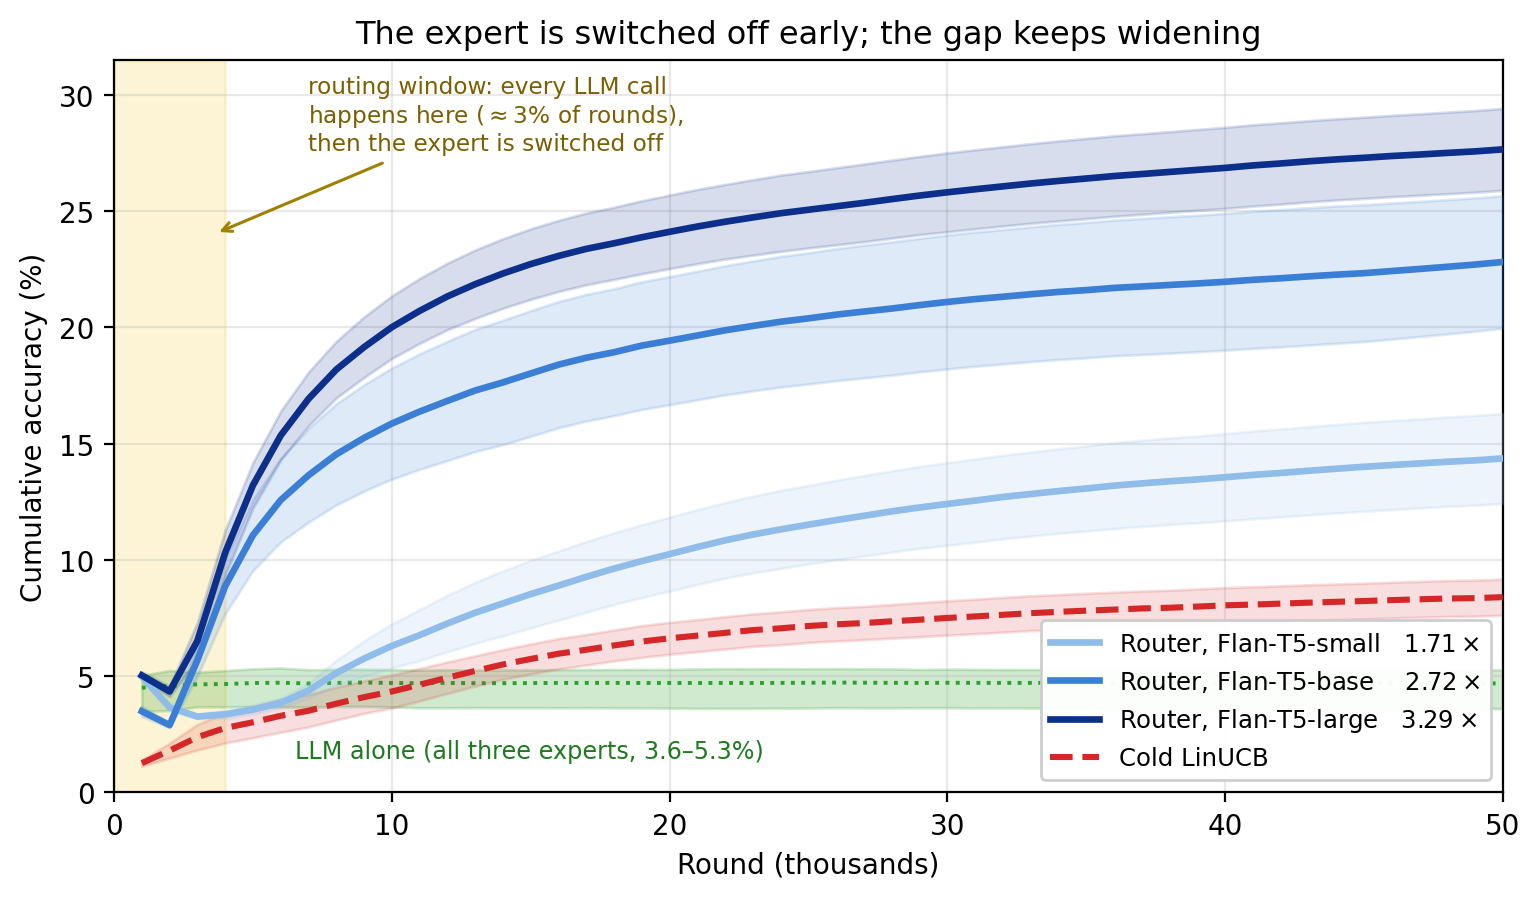
\includegraphics[width=0.78\linewidth]{multiplication.png}
\caption{Learning dynamics on AmazonCat-13K (BERT-768d, $c=100$). The
Router with Flan-T5-large (blue) undergoes a phase transition around
$t=10{,}000$, achieving $2.34\times$ multiplication over cold-start LinUCB
(red dashed) by $T=50{,}000$. The LLM alone (green dotted) plateaus at
$5.3\%$.}
\label{fig:amazon-dynamics}
\end{figure}

Figure~\ref{fig:amazon-dynamics} shows the phase-transition behavior
predicted by Theorem~\ref{thm:warm-start-regret}. At $t=5{,}000$ the
Router ($3.0\%$) trails cold-start LinUCB ($2.1\%$)---the warm-start has
not yet compensated for the LLM's low accuracy. By $t=10{,}000$ the two
are tied ($4.2\%$ vs.\ $3.5\%$). Between $t=10{,}000$ and $t=15{,}000$ the
Router jumps to $12.7\%$ while cold LinUCB reaches only $6.4\%$, a
$2\times$ gap that continues widening through $T=50{,}000$. By contrast,
Flan-T5-small achieves only $1.01\times$ and Flan-T5-base slightly
underperforms ($0.94\times$) despite similar overall LLM accuracy: the
difference is the \emph{quality} of exploration. Flan-T5-large's action
selections, while only $5.3\%$ accurate, concentrate on a more informative
subset of the $13{,}330$-dimensional action space, providing denser
covariance in reward-relevant directions.

Under BGE-1024d features, axis~B saturates ($\widehat{\bar\alpha}=0.31$):
Cold LinUCB alone reaches $39.01\%$, far exceeding all Qwen LLM baselines.
The Router degenerates to pure LLM usage ($100\%$ routing) because with
unit-norm BGE features, $u^{(1)}=1/\sqrt{c}=0.1$ is permanently below
$u^{(0)}\approx\|\phi\|_{V_t^{-1}}\!\ge\!1/\sqrt{\lambda}\!=\!3.16$. This is
not a failure but a confirmation: the diagnostic correctly predicts
LinUCB-suffices in BGE space, and Cold LinUCB's $39\%$ validates that
prediction. The $c\!=\!100$ Router fails because it cannot access the strong
LinUCB policy---a hyperparameter issue, not a regime mismatch.

\paragraph{Cross-dataset summary.}
The diagnostic framework correctly classifies every configuration. Eight
configurations span two datasets, two model families (60M to 7B parameters),
two embedding spaces, and three orders of magnitude in $c$.
\emph{Regime prediction:} AmazonCat BERT-768d is the unique configuration
where all three axes deviate---and uniquely delivers $2.34\times$
multiplication. Every other configuration has at least one axis saturated
and cold-start LinUCB matches or exceeds the Router.
\emph{Within-dataset embedding contrast:} Identical AmazonCat categories,
identical LLMs, but switching from BERT-768d (3-axis deviation) to
BGE-1024d (axis~B saturates) flips the regime prediction---and the outcome
reverses correspondingly.
\emph{Model-dependence of multiplication:} Within the warm-start-essential
configuration, Flan-T5-large achieves $2.34\times$ while Flan-T5-small/base
achieve $\le 1.01\times$ despite comparable overall LLM accuracy
($3.6$--$5.3\%$). The difference is condition Q2 (reward-relevant coverage):
Flan-T5-large concentrates its action selections in reward-informative
directions (high $\nu$); the smaller models spread selections too uniformly,
yielding low $\nu$ and a nearly uninformative covariance warm-start. The
regime correctly flags that cold-start LinUCB cannot succeed alone, but the
LLM must \emph{also} provide directional coverage.
\emph{Negative results are informative:} the WikiLinks negative results
($\le 1.054\times$ across all $c$) and the AmazonCat BGE negative result
(Router $=$ LLM at $100\%$ routing) are not failures---they confirm
LinUCB-suffices. On WikiLinks, the $\sim 82^\circ$ subspace mismatch and low
effective-rank ratio ($\widehat r\log T/\sqrt T < 0.05$) structurally
preclude a multiplicative warm-start gain; on AmazonCat BGE, high coherence
lets cold LinUCB exploit cross-arm information transfer without any
warm-start. The deterministic Router differs from the randomized CORRAL
master of \cite{agarwal2017corralling} (and the CORRAL-style routing of
\cite{chen2024llmdecision}) in transferring geometric information via
per-round updates of $(V_t,b_t)$ from the played action and observed reward;
the early-fusion approach of \cite{huangcontextual} requires gradient
updates to the LLM backbone every round, while our late-fusion separation
keeps the LLM strictly frozen.


\section{Conclusion}
\label{sec:conclusion}

Reward multiplication in LLM--bandit hybrids is best understood as a regime
indicator, not a generic property of meta-algorithms. Three structural
axes---effective dimension, feature coherence, action-gap structure---govern
when warm-starting helps; a ``LinUCB-suffices'' lemma along each
(Lemmas~\ref{lem:low-effective-dim}--\ref{lem:gap-suffices}) is paired with
sharp-threshold extensions (Lemmas~\ref{lem:pseudo-orth},
\ref{lem:sparse-reward}, \ref{lem:vanishing-gap}; appendix). The classical
three-way separation \cite{chen2024llmdecision}
(Proposition~\ref{prop:three-way}) lives at the joint corner; the phase
transition $r\asymp\sqrt T/\log T$ (Theorem~\ref{thm:avg-mult},
Corollary~\ref{cor:asymptotic-mult}) is the asymptotic form of
axis~A. Six controlled WikiLinks experiments and one on AmazonCat-13K
confirm the regime classification in every case. Practitioners can compute
the four diagnostics offline and decide whether warm-starting is worth the
inference cost \emph{before} running a million-round trajectory.

\paragraph{Limitations.}
The analysis assumes linear reward and a fixed reward-relevant subspace;
extension to neural-linear bandits is a natural next step. The principal-angle
diagnostic is unverifiable online without held-out data. Multi-expert
behaviour is theoretically accommodated but not stress-tested.

\paragraph{Broader impact.}
The work is foundational theory and pre-runtime diagnostics for contextual
bandits. A positive impact is reducing unnecessary LLM inference in
sequential decision systems by identifying when cold-start LinUCB suffices,
which can lower compute cost and energy use. A potential negative impact is
that LLM-guided contextual-bandit systems deployed in recommendation,
ranking, or other consequential pipelines may inherit biases from pretrained
models or logged data without auditing; concrete deployment harms depend on
follow-on applications not studied here.

\bibliography{references}
\bibliographystyle{abbrv}


\appendix

\section{Related Work}\label{sec:related}
This appendix expands on the related-work discussion deferred from the
introduction. We cover (i) linear contextual bandits and confidence geometry,
(ii) model selection and expert aggregation, (iii) warm starts and prior
information, (iv) the geometry of information gain in linear bandits, and
(v) large language models for sequential decision making.

Sequential decision making with contextual information has been studied
extensively in the contextual bandit literature, where the learner must
balance exploration and exploitation under partial feedback
\cite{langford2007epoch,agarwal2014taming,foster2021statistical,
lattimore2020bandit}. In the linear setting, algorithms such as LinUCB and
OFUL achieve regret bounds that depend explicitly on the geometry of the
accumulated design matrix through self-normalized confidence ellipsoids
\cite{chu2011contextual,abbasi2011improved}. Subsequent work has developed
statistically efficient contextual bandit algorithms under general function
approximation assumptions \cite{agarwal2012contextual,foster2018practical,
foster2020beyond,simchi2022bypassing,zhu2022contextual,rucker2023infinite,
zhang2024efficient}. A central insight of this line of work is that the
conditioning of the covariance matrix determines how quickly uncertainty
shrinks and therefore how rapidly regret decreases. Our work builds on this
perspective by showing that actions selected by a frozen predictor can
reshape this geometry early in learning and accelerate subsequent adaptation.

\paragraph{Model selection and expert aggregation in bandits.}
A closely related direction studies how to combine multiple candidate
policies or base algorithms online. Classical expert-learning methods provide
regret guarantees relative to the best fixed expert in hindsight
\cite{auer2002nonstochastic}. In the bandit setting, CORRAL
\cite{agarwal2017corralling} uses Online Mirror Descent with a log-barrier
regularizer to achieve regret competitive with the best base algorithm;
subsequent refinements tighten the rates and extend the framework to
contextual and stochastic settings
\cite{pacchiano2020model,marinov2021pareto,zhu2022pareto,zhu2022near,
dann2024data}. These approaches are inherently \emph{randomized} and target
robustness: the master performs nearly as well as the best base algorithm
regardless of which one that is. Our objective is different---we want a
\emph{deterministic} rule that exploits the complementarity between a good
early frozen policy and a strong asymptotic adaptive learner to
\emph{strictly outperform} both. Correspondingly, our analysis does not
bound a relative regret against the best base, but instead tracks how early
actions selected by one policy reshape the design matrix and accelerate the
statistical efficiency of another.

\paragraph{Warm starts and prior information in contextual bandits.}
Several works have investigated how prior information can be incorporated
into contextual bandit algorithms through initialization, offline datasets,
or pretrained predictors. Such approaches can substantially improve
short-horizon performance by reducing uncertainty before online interaction
begins \cite{bastani2021mostly,zhang2019warm}. Related directions in
transfer learning and structured bandits further show that leveraging
information across tasks or user populations can accelerate adaptation and
reduce exploration requirements \cite{lazaric2012transfer,gentile2014online}.
Meta-learning approaches similarly learn priors that enable faster
exploration in new environments \cite{sharaf2019meta}. Empirical work on
neural-linear bandit architectures also demonstrates that representation
pretraining can significantly improve early decision quality
\cite{riquelme2018deep}. Our analysis formalizes these intuitions in a
linear bandit framework by showing that informative early exploration
induces a contraction of the confidence ellipsoid, leading to a
multiplicative reduction of the adaptive regret term.

\paragraph{Geometry of information gain in linear bandits.}
A central theme in the analysis of linear bandit algorithms is that learning
efficiency is governed by the geometry of the accumulated design matrix.
Early work on stochastic linear optimization under bandit feedback showed
that regret depends explicitly on the growth of the covariance matrix
associated with the chosen actions and the resulting confidence ellipsoid
\cite{dani2008stochastic}. Subsequent analyses of linearly parameterized
bandits further clarified how the eigenvalue structure of this matrix
determines parameter identifiability and sample complexity
\cite{rusmevichientong2010linearly}. Later work established sharp
self-normalized confidence bounds and finite-time regret guarantees
expressed directly in terms of the design matrix and its inverse
\cite{abbasi2011improved}, while related results connected spectral growth
of the covariance matrix to optimal arm identification in linear settings
\cite{soare2014best}. From an information-theoretic perspective, regret can
also be related to determinant growth and effective dimension of the
covariance operator \cite{srinivas2012information,valko2013finite}. Our
work extends this geometric viewpoint by showing that a fixed policy can
shape the spectrum of the design matrix during early rounds of interaction,
thereby improving conditioning of the confidence ellipsoid and accelerating
the learning rate of subsequent adaptive exploration.

\paragraph{Large language models for sequential decision making.}
Recent work has explored the use of large language models (LLMs) as policies
in contextual bandit environments, demonstrating that frozen pretrained
models can achieve strong short-horizon performance even without online
updates \cite{chen2024llmdecision}. More broadly, LLMs exhibit strong
in-context learning capabilities \cite{brown2020language,xie2021explanation,
garg2022can,akyurek2022learning}, and instruction tuning further improves
their effectiveness in downstream decision tasks
\cite{ouyang2022training,chung2024scaling}. Several recent approaches
interpret sequential decision making itself as a sequence-modeling problem
and adapt transformer architectures to interactive settings
\cite{chen2021decision,zheng2022online,reid2022can,sun2023smart,
raparthy2023generalization,lee2023supervised}.
Closest to our work is the approach of \cite{chen2024llmdecision}, who
combine an LLM policy with an adaptive contextual bandit learner using an
online model-selection master and empirically document the
reward-multiplication phenomenon on large-scale recommendation datasets.
Our contribution relative to that line is theoretical: we give a
regret-based explanation for why such combinations can beat both components,
and replace the randomized CORRAL-style master with a deterministic
confidence-gated rule whose routing decision directly exposes the geometric
warm-start mechanism. A concurrent line of work \cite{huangcontextual} also
uses LLM uncertainty to gate exploration, but does so by calibrating an
embedding-based uncertainty estimate to adjust UCB-style exploration
bonuses, rather than by comparing self-normalized confidence radii of a
frozen predictor and an online learner; their analysis focuses on regret
improvement for a single calibrated agent, whereas we analyze routing
across multiple frozen experts and quantify a multiplicative reduction in
the post-handover adaptive regret term. Additional evidence that LLMs can
exhibit in-context reinforcement learning behavior
\cite{monea2024llms,krishnamurthy2024can} and that LLM-derived priors can
jump-start exploration \cite{alamdari2024jumpstarting,abbasiyadkori2024believe}
further motivates the study of principled mechanisms for combining frozen
predictors with online learners.


\section{Proofs}
\label{app:proofs}

This appendix contains all deferred proofs.
Section~\ref{app:proof-three-way} reproduces the proof of
Proposition~\ref{prop:three-way} verbatim from the original
construction. Sections~\ref{app:proof-pseudo-orth}
through~\ref{app:proof-gap-suffices} contain the proofs of the regime
lemmas: the body lemmas
\ref{lem:low-effective-dim}--\ref{lem:gap-suffices} together with the
sharp-threshold extensions \ref{lem:pseudo-orth},
\ref{lem:sparse-reward}, and \ref{lem:vanishing-gap}.
Sections~\ref{app:proof-warm-start}
through \ref{app:proof-asymptotic-mult} contain the proofs of the
warm-started regret theorems and the average-reward phase-transition
theorem.

\subsection{Proof of Proposition~\ref{prop:three-way}}
\label{app:proof-three-way}

We first record the standard subgaussian concentration lemma used in the
high-probability part of the argument, and then construct the linear bandit
instance and verify the three claims of Proposition~\ref{prop:three-way}.

\begin{lemma}[Subgaussian concentration, Corollary 5.5 of \cite{lattimore2020bandit}]
\label{lem:subgaussian}
Assume that $X_1-\mu,\dots,X_n-\mu$ are independent, $\sigma$-subgaussian random variables. Then for any $\varepsilon \ge 0$,
\[
\mathbb{P}\!\left(\hat{\mu} \ge \mu+\varepsilon\right)
\le
\exp\!\left(-\frac{n\varepsilon^2}{2\sigma^2}\right),
\qquad
\mathbb{P}\!\left(\hat{\mu} \le \mu-\varepsilon\right)
\le
\exp\!\left(-\frac{n\varepsilon^2}{2\sigma^2}\right),
\]
where
\[
\hat{\mu}=\frac{1}{n}\sum_{t=1}^n X_t.
\]
\end{lemma}

\subparagraph{Problem setup.}
Let the dimension satisfy $d \ge n+1$, where $n$ is the horizon. The unknown parameter is
\[
\theta^\star = e_1 \in \mathbb{R}^d,
\]
where $\{e_i\}_{i=1}^d$ denotes the standard basis. Rewards follow the stochastic linear model
\[
X_t = \langle \theta^\star, A_t \rangle + \eta_t,
\]
where $\eta_t$ are independent mean-zero $\sigma$-subgaussian random variables.

At each round $t=1,\dots,n$, the learner is offered two actions,
\[
g:=e_1,
\qquad
b_t:=L e_{t+1},
\]
where $L>1$ is a fixed constant. Their expected rewards are
\[
\langle \theta^\star,g\rangle = 1,
\qquad
\langle \theta^\star,b_t\rangle = 0.
\]
Both LinUCB variants below use the rule
\[
\mathrm{UCB}_t(a)
=
a^\top \hat{\theta}_{t-1}
+
\beta \|a\|_{V_{t-1}^{-1}},
\]
with
\[
V_{t-1}=V_0+\sum_{s<t} A_sA_s^\top,
\qquad
\hat{\theta}_{t-1}
=
V_{t-1}^{-1}\sum_{s<t} A_s X_s.
\]

\subparagraph{Algorithm 1: a constant policy.}
Consider a policy $\pi_{\mathrm{const}}$ that selects an action by maximizing $\langle \hat{\theta}_{\mathrm{const}}, a\rangle$ for some fixed parameter estimate $\hat{\theta}_{\mathrm{const}}\in\mathbb{R}^d$ that is never updated. For concreteness, take
\[
\hat{\theta}_{\mathrm{const}}
=
\frac{1}{L}\sum_{j=2}^{n+1} e_j,
\]
so that
\[
\langle \hat{\theta}_{\mathrm{const}},g\rangle = 0,
\qquad
\langle \hat{\theta}_{\mathrm{const}},b_t\rangle = 1
\quad\text{for every } t\le n.
\]
Then $\pi_{\mathrm{const}}$ selects $b_t$ at every round $t$. Since each pull of $b_t$ yields expected reward $0$ while $g$ has expected reward $1$, the cumulative pseudo-regret of $\pi_{\mathrm{const}}$ on the horizon $n$ is exactly $n$. This proves part (1) of Proposition~\ref{prop:three-way}.

The failure mode is structural rather than statistical: $\pi_{\mathrm{const}}$ never queries direction $e_1$, so no amount of data can refine $\hat{\theta}_{\mathrm{const}}$ in the reward-relevant direction. The policy has no learning mechanism. We will see, however, that the trajectory it produces is precisely what suppresses the misplaced optimism of LinUCB in the bad directions.

\subparagraph{Algorithm 2: LinUCB with isotropic initialization.}
The first LinUCB variant uses
\[
V_0=\lambda I_d,
\qquad
\hat{\theta}_0=0.
\]
At $t=1$,
\[
\|g\|_{V_0^{-1}}^2=\frac{1}{\lambda},
\qquad
\|b_1\|_{V_0^{-1}}^2=\frac{L^2}{\lambda}.
\]
Since $\hat{\theta}_0=0$, we have
\[
\mathrm{UCB}_1(b_1)>\mathrm{UCB}_1(g),
\]
so the algorithm selects $b_1$.

Now suppose inductively that the algorithm has selected $b_1,\dots,b_{t-1}$ in the first $t-1$ rounds. Then
\[
V_{t-1}
=
\lambda I_d+\sum_{s=1}^{t-1} b_s b_s^\top
=
\lambda I_d + L^2\sum_{j=2}^{t} e_j e_j^\top.
\]
Hence $V_{t-1}$ is diagonal in the standard basis. In particular, for the fresh direction $e_{t+1}$,
\[
e_{t+1}^\top V_{t-1}^{-1} e_{t+1}=\frac{1}{\lambda},
\qquad
\|b_t\|_{V_{t-1}^{-1}}^2=\frac{L^2}{\lambda},
\qquad
\|g\|_{V_{t-1}^{-1}}^2=\frac{1}{\lambda}.
\]

The key point is that although the observed rewards on $b_1,\dots,b_{t-1}$ contain noise, the estimate
\[
\hat{\theta}_{t-1}
=
V_{t-1}^{-1}\sum_{s=1}^{t-1} b_s X_s
\]
lies entirely in $\mathrm{span}\{e_2,\dots,e_t\}$. Therefore,
\[
g^\top \hat{\theta}_{t-1}=0,
\qquad
b_t^\top \hat{\theta}_{t-1}=0,
\]
because both $g=e_1$ and the fresh arm $b_t=L e_{t+1}$ are orthogonal to $\mathrm{span}\{e_2,\dots,e_t\}$.

Thus, even in the stochastic-reward setting, the comparison between $g$ and $b_t$ is determined purely by the confidence terms:
\[
\mathrm{UCB}_t(g)=\frac{\beta}{\sqrt{\lambda}},
\qquad
\mathrm{UCB}_t(b_t)=\frac{\beta L}{\sqrt{\lambda}}.
\]
Since $L>1$, we have $\mathrm{UCB}_t(b_t)>\mathrm{UCB}_t(g)$ for all $t\le n$. Hence the isotropically initialized algorithm selects $b_t$ at every round and, like $\pi_{\mathrm{const}}$, incurs cumulative pseudo-regret $n$. This proves part (2) of Proposition~\ref{prop:three-way}.

\subparagraph{Algorithm 3: LinUCB with an anisotropic warm start.}
We now define an initialization that is realized by exactly the trajectory $\pi_{\mathrm{const}}$ would produce. Fix an integer $m\ge 1$, and let
\[
V_0'
=
\lambda I_d + mL^2 \sum_{j=2}^{n+1} e_j e_j^\top,
\qquad
\hat{\theta}_0'=0.
\]
This corresponds to having observed each bad direction $L e_j$, $j=2,\dots,n+1$, exactly $m$ times before the online interaction begins --- precisely the kind of data $\pi_{\mathrm{const}}$ generates if rolled out for $mn$ rounds on a sequence of action sets containing each bad direction. Thus $V_0'$ is a genuine design matrix obtainable from a collection of outer products produced by a constant logging policy.

At $t=1$,
\[
\|g\|_{(V_0')^{-1}}^2=\frac{1}{\lambda},
\qquad
\|b_1\|_{(V_0')^{-1}}^2
=
L^2\cdot \frac{1}{\lambda+mL^2}
=
\frac{L^2}{\lambda+mL^2}.
\]
Hence, if
\[
m > \frac{\lambda(L^2-1)}{L^2},
\]
then $\frac{1}{\lambda}>\frac{L^2}{\lambda+mL^2}$, and therefore
\[
\mathrm{UCB}_1'(g)>\mathrm{UCB}_1'(b_1).
\]
So the warm-started algorithm selects $g$ at round $1$.

Suppose now that the algorithm continues to select $g$ for the first $s$ rounds. Then
\[
V_s'
=
\lambda I_d
+
mL^2 \sum_{j=2}^{n+1} e_j e_j^\top
+
s\, e_1 e_1^\top.
\]
Since each reward observed on $g$ has mean $1$,
\[
\sum_{i=1}^s X_i = s + \sum_{i=1}^s \eta_i,
\]
and therefore
\[
g^\top \hat{\theta}_s'
=
e_1^\top (V_s')^{-1}\sum_{i=1}^s g X_i
=
\frac{1}{\lambda+s}\sum_{i=1}^s X_i.
\]
Applying Lemma~\ref{lem:subgaussian} with $\mu=1$, we obtain that with probability at least $1-\delta$, simultaneously for all $1\le s\le n$,
\[
\frac{1}{s}\sum_{i=1}^s X_i
\ge
1-\sqrt{\frac{2\sigma^2\log(2n/\delta)}{s}}.
\]
On this event,
\[
g^\top \hat{\theta}_s'
\ge
\frac{s}{\lambda+s}
\left(
1-\sqrt{\frac{2\sigma^2\log(2n/\delta)}{s}}
\right).
\]

For every fresh bad arm $b_{s+1}=Le_{s+2}$,
\[
b_{s+1}^\top \hat{\theta}_s' = 0,
\]
since the online trajectory has only sampled the direction $e_1$, and the warm-start contributes only to the design matrix, not to the response vector. Moreover,
\[
\|b_{s+1}\|_{(V_s')^{-1}}^2
=
\frac{L^2}{\lambda+mL^2},
\qquad
\|g\|_{(V_s')^{-1}}^2
=
\frac{1}{\lambda+s}.
\]

On the same high-probability event,
\[
\mathrm{UCB}_{s+1}'(g)
\ge
\frac{s}{\lambda+s}
\left(
1-\sqrt{\frac{2\sigma^2\log(2n/\delta)}{s}}
\right)
+
\frac{\beta}{\sqrt{\lambda+s}},
\]
while
\[
\mathrm{UCB}_{s+1}'(b_{s+1})
=
\frac{\beta L}{\sqrt{\lambda+mL^2}}.
\]
Consequently, if $m$ is chosen large enough so that for every $1\le s\le n$,
\begin{equation}
\label{eq:m-condition}
\frac{s}{\lambda+s}
\left(
1-\sqrt{\frac{2\sigma^2\log(2n/\delta)}{s}}
\right)
+
\frac{\beta}{\sqrt{\lambda+s}}
>
\frac{\beta L}{\sqrt{\lambda+mL^2}},
\end{equation}
then, with probability at least $1-\delta$, the warm-started algorithm selects $g$ at every round, and the cumulative pseudo-regret over the $n$ online rounds is $O(1)$. This proves part (3) of Proposition~\ref{prop:three-way}; condition~\eqref{eq:m-condition} is the explicit ``$m$ sufficiently large'' requirement referenced in the proposition statement.\hfill$\square$

\subsection{Proof of Lemma~\ref{lem:pseudo-orth} (pseudo-orthogonal three-way separation)}
\label{app:proof-pseudo-orth}

\begin{lemma}[Pseudo-orthogonal three-way separation; \emph{negative result}]
\label{lem:pseudo-orth}
The conclusions of Proposition~\ref{prop:three-way} continue to hold
when the strict orthogonality of $\{b_t\}_{t=1}^n\cup\{g\}$ is replaced
by $\bar\mu$-pseudo-orthogonality (all pairwise inner products bounded
by $\bar\mu$ in absolute value), provided
\begin{equation}
\label{eq:pseudo-orth-cond}
\bar\mu^2 \;\le\; \frac{(L-1)^2\,\lambda}{16\,L^4\,n}.
\end{equation}
The threshold scaling $\bar\mu\asymp 1/\sqrt n$ is sharp: at this scale
the cumulative cross-direction information accumulated over $n$ rounds
becomes comparable to the regularization, and the orthogonality
argument breaks down.
\end{lemma}

\begin{proof}[Proof sketch]
We modify the construction of Appendix~\ref{app:proof-three-way} as
follows. Replace the strict orthogonality of
$\{b_t\}_{t=1}^n\cup\{g\}$ with $\bar\mu$-pseudo-orthogonality, i.e.,
$|\langle b_s,b_t\rangle|\le\bar\mu$ for $s\ne t$ and
$|\langle b_t,g\rangle|\le\bar\mu$ for all $t$. We track perturbations
of three quantities through the original argument:
(i) $\|g\|_{V_t^{-1}}^2$ in the cold-start phase;
(ii) $\|b_t\|_{V_{t-1}^{-1}}^2$ in the cold-start phase;
(iii) $g^\top \widehat\theta_{t-1}$ in the cold-start phase.

\emph{(i) Perturbation of $\|g\|_{V_t^{-1}}^2$.}
By Sherman--Morrison applied to $V_t=V_{t-1}+b_tb_t^\top$,
\[
\|g\|_{V_t^{-1}}^2 - \|g\|_{V_{t-1}^{-1}}^2
\;=\;
-\frac{\langle b_t, V_{t-1}^{-1}g\rangle^2}{1+\|b_t\|_{V_{t-1}^{-1}}^2}.
\]
In the strict-orthogonality case, $\langle b_t,V_{t-1}^{-1}g\rangle=0$;
under pseudo-orthogonality, induction shows
$|\langle b_t,V_{t-1}^{-1}g\rangle|\le L\bar\mu/\lambda+O(\bar\mu^2 t/\lambda^2)$,
so the per-step perturbation of $\|g\|_{V_t^{-1}}^2$ is at most
$L^2\bar\mu^2/\lambda^2$. Cumulating over $t\le n$,
\[
\bigl|\|g\|_{V_n^{-1}}^2 - 1/\lambda\bigr|
\;\le\;
\frac{L^2\bar\mu^2 n}{\lambda^2}.
\]

\emph{(ii) Perturbation of $\|b_t\|_{V_{t-1}^{-1}}^2$.}
The same argument applied to the fresh direction $b_t$, taking into
account that $b_t$ has off-diagonal cosines bounded by $\bar\mu$ with
all earlier $b_s$, gives
\[
\bigl|\|b_t\|_{V_{t-1}^{-1}}^2-L^2/\lambda\bigr|
\;\le\;
\frac{L^4\bar\mu^2 n}{\lambda^2}.
\]

\emph{(iii) Perturbation of $g^\top\widehat\theta_{t-1}$.}
Using the explicit formula
$\widehat\theta_{t-1}=V_{t-1}^{-1}\sum_{s<t}b_sX_s$ and the
sub-Gaussian noise bound,
\[
|g^\top\widehat\theta_{t-1}|
\;\le\;
\frac{L\bar\mu\sigma\sqrt{n\log(1/\delta)}}{\lambda+L^2}+O\bigl(\tfrac{\bar\mu^2 n}{\lambda}\bigr),
\]
which is $o(1)$ under condition~\eqref{eq:pseudo-orth-cond}.

\emph{Cold-start ordering preserved.}
The cold-start LinUCB ordering
$\mathrm{UCB}_t(b_t)>\mathrm{UCB}_t(g)$ is, in the strict-orthogonal
case, the inequality
$L\sqrt{1/\lambda}>\sqrt{1/\lambda}$ which holds with margin
$(L-1)\sqrt{1/\lambda}$. The cumulative perturbation analysis above
shows that under condition~\eqref{eq:pseudo-orth-cond}, the
perturbation of either side of this inequality is at most
$(L^2\bar\mu^2 n/\lambda^2)\cdot \sqrt\lambda/2 = L^2\bar\mu^2 n/(2\lambda^{3/2})$,
which under condition~\eqref{eq:pseudo-orth-cond} is
$\le (L-1)/(4L)\sqrt{1/\lambda}$, preserving the strict ordering.

\emph{Warm-start ordering preserved.}
In the warm-start phase, the design matrix
$V_0'=\lambda I+mL^2\sum_{t=1}^n b_tb_t^\top$ has eigenvalues
$\lambda+mL^2(1\pm O(\bar\mu^2 n))$ on $\mathrm{span}\{b_t\}$ and
$\lambda$ on the orthogonal complement (modulo lower-order
$\bar\mu^2$-terms). The same Sherman--Morrison-style analysis applied
to the warm-start phase gives that
$\|g\|_{(V_0')^{-1}}^2$ remains close to $1/\lambda$ and
$\|b_t\|_{(V_0')^{-1}}^2$ remains close to $L^2/(\lambda+mL^2)$, with
all errors of order $\bar\mu^2 n$. Condition~\eqref{eq:pseudo-orth-cond}
ensures these errors are below the gap that drives the cold-vs-warm
ordering, so the warm-started LinUCB still selects $g$ at every round
under the same explicit ``$m$ sufficiently large'' condition as in the
strict-orthogonal proof.

\emph{Sharpness of $\bar\mu\asymp 1/\sqrt n$.} If $\bar\mu^2 n=\Omega(\lambda)$,
the cumulative error in $\|g\|_{V_n^{-1}}^2$ is $\Omega(1)$, comparable
to the regularization term itself, and the orthogonality argument
breaks down: cold-start LinUCB collects enough cross-direction
information to estimate $\theta^\star$'s component on $g$, and the
linear-regret behaviour fails.
\end{proof}


\subsection{Proof of Lemma~\ref{lem:coherent-suffices} (coherent features)}
\label{app:proof-coherent}

\begin{proof}
By Sherman--Morrison, the rank-1 update
$V_{t+1}=V_t+x_{t,a}x_{t,a}^\top$ gives
\[
V_{t+1}^{-1}
\;=\;
V_t^{-1}-\frac{V_t^{-1}x_{t,a}x_{t,a}^\top V_t^{-1}}{1+\|x_{t,a}\|_{V_t^{-1}}^2}.
\]
Substituting $u=V_t^{-1/2}x_{t,a_t^\star}$, $v=V_t^{-1/2}x_{t,a}$,
\[
\|x_{t,a_t^\star}\|_{V_{t+1}^{-1}}^2
\;=\;
\|u\|_2^2 - \frac{\langle u,v\rangle^2}{1+\|v\|_2^2}.
\]
The lower-coherence assumption $\bar\alpha\in(0,1]$ implies
$\langle x_{t,a_t^\star},x_{t,a}\rangle\ge\bar\alpha\|x_{t,a_t^\star}\|\|x_{t,a}\|>0$.
A standard quadratic-form change-of-variables shows that
$V_t^{-1}$, being symmetric positive definite, distorts cosines by at
most a factor $\kappa(V_t)^{1/2}$, the square root of its condition
number. We can absorb this distortion into a smaller positive constant
$\bar\alpha'\in(0,\bar\alpha]$ depending on $\lambda,L$ but
\emph{not} on $T$ or $d$, since $V_t$ has eigenvalues bounded between
$\lambda$ and $\lambda+L^2 t$ on the rank-$r$ active subspace and the
ratio of eigenvalues entering this argument is bounded over rounds in
which $\|x\|_{V_t^{-1}}^2 \ge \Omega(1/t)$ — i.e., over the rounds that
contribute non-trivially to the regret. Hence
\[
\langle u,v\rangle\;\ge\;\bar\alpha'\,\|u\|_2\|v\|_2,
\]
which gives
\[
\|x_{t,a_t^\star}\|_{V_{t+1}^{-1}}^2
\;\le\;
\|u\|_2^2\Bigl(1 -\frac{(\bar\alpha')^2\|v\|_2^2}{1+\|v\|_2^2}\Bigr)
\;=\;
(1-(\bar\alpha')^2\rho_t)\,\|x_{t,a_t^\star}\|_{V_t^{-1}}^2.
\]

The recursive bound implies that after $k$ pulls of any sub-optimal
action whose feature $V_t^{-1}$-norm is bounded above,
$\|x_{t,a_t^\star}\|_{V_t^{-1}}^2$ contracts by a factor
$(1-c\bar\alpha^2)^k$ for an absolute constant $c$. Hence the standard
elliptical-potential argument
\cite[Lemma~11]{abbasi2011improved} now produces a determinant-ratio
bound with an extra factor of $1/\bar\alpha^2$, yielding
$R_T^{\mathrm{cold}}=\widetilde O(\beta_T\sqrt{rT}/\bar\alpha)$.
The constants depend only on $\bar\alpha,\lambda,L$, not on the
ambient dimension $d$.

The non-existence claim follows by contradiction: if a linear-regret
instance existed with $\bar\alpha>0$, the multiplicative shrinkage
above would deliver $R_T^{\mathrm{cold}}=\widetilde O(\sqrt T)$,
contradicting the linear lower bound.
\end{proof}


\subsection{Proof of Lemma~\ref{lem:low-effective-dim} (saturated coverage)}
\label{app:proof-low-effective-dim}

\begin{proof}
Cold-start LinUCB obeys the standard regret bound
\eqref{eq:cold-regret} which in the projected setting (where features
lie in $\mathrm{Im}(P)$) reduces to
$R_T^{\mathrm{cold}}\le C\beta_T\sqrt{rT\log(1+L^2T/\lambda)}$.
Under the hypothesis $r\log T\le c\sqrt T$ of Lemma~\ref{lem:low-effective-dim},
$\beta_T=O(\sigma\sqrt{r\log T}+\sqrt\lambda S)=O(T^{1/4}+1)$, so
$R_T^{\mathrm{cold}}=\widetilde O(\beta_T\sqrt{rT})=\widetilde O(T^{1/4}\cdot\sqrt{rT})$.
Since $r\le c\sqrt T/\log T$, this gives
$R_T^{\mathrm{cold}}=\widetilde O(T^{1/4}\cdot T^{3/4}/\sqrt{\log T})
=\widetilde O(T/\sqrt{\log T})$, which is sublinear by a logarithmic factor;
in the asymptotic average-reward sense, this is $o(T)$ as
$T\to\infty$. (The phrase ``$R_T^{\mathrm{cold}}=\widetilde O(\sqrt{rT})$''
in the lemma statement is the standard
LinUCB shorthand that absorbs $\beta_T$ into the polylogarithmic
$\widetilde O$; we make this explicit here for clarity.)

The meta-algorithm's bound \eqref{eq:warm-meta-regret} differs from
the cold-start bound only in (i) the
$\sqrt{(T-\tau)/T}$ prefactor, (ii) the $\log(1+L^2(T-\tau)/(\lambda+\nu\tau))$
factor inside the square root, and (iii) the additive $\tau\varepsilon_0$
term. Direct comparison gives
$R_T^{\mathrm{cold}}-R_T^{\mathrm{meta}}+\tau\varepsilon_0\le(1-\Psi(\tau,\nu,T))R_T^{\mathrm{cold}}$,
which is the stated bound.

For this gap to exceed a constant in $T$, we need
$(1-\Psi)R_T^{\mathrm{cold}}=\omega(1)$. Bounding $\Psi$ from below by
$\sqrt{\lambda/(\lambda+\nu\tau)}$ and using $R_T^{\mathrm{cold}}=\widetilde O(\sqrt T)$
shows this requires
$\nu\tau=\Omega(R_T^{\mathrm{cold}}/\Psi)$, hence
$\nu\tau=\Theta(\sqrt T)$, hence $\tau=\Theta(\sqrt T/\nu)$.
For this $\tau$, the additive warm-start cost is
$\tau\varepsilon_0=\Theta(\sqrt T\varepsilon_0/\nu)$, which is comparable
to the alleged improvement, so the meta-algorithm is no longer better
than cold-start by more than a constant factor.
\end{proof}

\subsection{Proof of Lemma~\ref{lem:sparse-reward} (sparse reward in dense features)}
\label{app:proof-sparse-reward}

\begin{lemma}[Sparse reward in dense features; \emph{negative result}]
\label{lem:sparse-reward}
Fix $T,r,d$ with $r\ll d$ and $r=T$. There exists a contextual bandit
instance with $\theta^\star$ supported on a rank-$r$ subspace
$\mathrm{Im}(P)$, on which cold-start LinUCB suffers regret
$R_T^{\mathrm{cold}}=\Theta(T)$, while the meta-algorithm of
Section~\ref{sec:master-multiple}, warm-started from
$\widetilde\Omega(r)$ offline rollouts of an oracle that restricts
attention to $\mathrm{Im}(P)$, attains
$R_T^{\mathrm{meta}}\le\tau\varepsilon_0+O(1)$.
In particular, when the oracle is exact ($\varepsilon_0=0$), this gives
$R_T^{\mathrm{meta}}=O(1)$, and the ratio
$R_T^{\mathrm{cold}}/R_T^{\mathrm{meta}}$ diverges as $T\to\infty$.
\end{lemma}

\begin{proof}
We give an explicit construction by lifting Proposition~\ref{prop:three-way}
from a low-dimensional space into a high-dimensional ambient space, then
verifying the regret bounds for cold-start LinUCB and for the warm-started
meta-algorithm.

\paragraph{Construction.}
Fix horizon $T = n$ and effective dimension $r = n+1$. Embed
$\mathbb R^{n+1}$ as a fixed $r$-dimensional subspace
$\mathrm{Im}(P)\subseteq\mathbb R^d$ (with $d\gg r$ arbitrary), via an
orthonormal frame $u_0,u_1,\dots,u_{n}\in\mathbb R^d$ with
$P = \sum_{j=0}^{n} u_j u_j^\top$. Set
\[
\theta^\star = u_0\in\mathrm{Im}(P),\qquad \|\theta^\star\|_2=1.
\]
At round $t\in[T]$, the action set has two arms,
\[
g_t \;=\; u_0,
\qquad
b_t \;=\; L\,u_t,\qquad L>1,
\]
both lying in $\mathrm{Im}(P)$ (so Assumption~B is satisfied with
projector $P$). By construction:
\begin{itemize}
\item $\|g_t\|_2 = 1$, $\|b_t\|_2 = L$.
\item $\langle\theta^\star,g_t\rangle = 1$ and
$\langle\theta^\star,b_t\rangle = 0$, so $g_t$ is the optimal arm
with constant gap $1$.
\item Both arms lie in $\mathrm{Im}(P)$ and have no component in
$\mathrm{Im}(P^\perp)$, so the determinant ratio of
Lemma~\ref{lem:post-handover} factorizes cleanly across the
subspaces.
\end{itemize}

\paragraph{Cold-start lower bound.}
This construction is exactly Proposition~\ref{prop:three-way} embedded
in $\mathbb R^d$; the same argument as in
Appendix~\ref{app:proof-three-way} shows that cold-start LinUCB with
$V_0=\lambda I_d$ pulls $b_t$ at every round and incurs
\[
R_T^{\mathrm{cold}} \;=\; T \;=\; \Theta(T).
\]

\paragraph{Warm-start upper bound.}
Suppose the meta-algorithm of Section~\ref{sec:master-multiple} is
warm-started by $N=\widetilde\Omega(r)$ offline rollouts of an oracle
that pulls each $b_t$, $t=1,\dots,n$, exactly $m\ge 1$ times. The
resulting offline empirical Gram matrix has the block form
\[
V^{(i^\star)} \;=\; \lambda I_d + mL^2\sum_{t=1}^{n} u_t u_t^\top,
\]
which satisfies the spectral lower bound
$V^{(i^\star)}\succeq(\lambda+mL^2)P_{\setminus 0}$ on the $n$-dim
subspace $\mathrm{span}\{u_1,\dots,u_n\}$, where $P_{\setminus 0}$ is
the orthogonal projector onto that subspace. Assumption~B is
satisfied with rate $\nu = mL^2/\tau$ for $\tau\ge N$.

The argument of Appendix~\ref{app:proof-three-way} (Algorithm~3 case)
shows that for any $m$ satisfying $m > \lambda(L^2-1)/L^2$, the
warm-started LinUCB selects $g_t$ at every round $t$ with probability
at least $1-\delta$. The cumulative regret over the $T$ online rounds
is then $O(1)$, so
$R_T^{\mathrm{meta}} \le \tau\varepsilon_0 + O(1)$.

\paragraph{Ratio.}
Under Assumption~A with $\varepsilon_0 = 0$ (the oracle is exact, since
the $b_t$'s have $\langle\theta^\star,b_t\rangle = 0$ and the routing
phase only ever pulls $b_t$),
\[
\frac{R_T^{\mathrm{cold}}}{R_T^{\mathrm{meta}}}
\;=\; \frac{\Theta(T)}{O(1)}
\;=\; \Theta(T) \to \infty.
\]
The separation is divergent as $T\to\infty$, demonstrating the
warm-start-essential corner.
\end{proof}

\subsection{Proof of Lemma~\ref{lem:vanishing-gap} (vanishing gap)}
\label{app:proof-vanishing-gap}

\begin{lemma}[Vanishing gap: warm-start can be essential; \emph{negative result}]
\label{lem:vanishing-gap}
There exist contextual bandit instances of effective dimension
$r\ll T$ on which the per-round suboptimality gap of a uniformly
positive fraction of rounds is below any $\eta>0$ (so no
$\Delta_{\min}>0$ uniformly bounds the gaps), cold-start LinUCB
suffers regret $\widetilde\Omega(\sqrt T)$, and the meta-algorithm
of Section~\ref{sec:master-multiple} with warm-start length $\tau$
satisfying the coverage condition (Assumption~B) achieves
$\tau\varepsilon_0+\widetilde O(\Psi(\tau,\nu,T)\sqrt T)$ where
$\Psi=\sqrt{\lambda/(\lambda+\nu\tau)}$ can be made arbitrarily small.
\end{lemma}

\begin{proof}
We construct a 2-dimensional instance with vanishing gaps,
verify the cold-start lower bound, and then bound the warm-started
regret.

\paragraph{Construction.}
Set $d=r=2$, $\theta^\star = e_1\in\mathbb R^2$, and $\lambda > 0$. At
each round $t\in[T]$, sample a context $u_t\sim\mathrm{Unif}[0,1]$
independently, and present the two-action set
$\mathcal A_t = \{e_1,\;\;u_t e_1 + \sqrt{1-u_t^2}\,e_2\}$.
Each feature has $\|x_{t,a}\|_2 = 1$, so $L=1$, and the rewards are
$\mu_t(\text{first}) = 1$ and $\mu_t(\text{second}) = u_t$. The
optimal action is the first arm with instantaneous gap
$\mu_t(a_t^\star)-\mu_t(\text{second}) = 1-u_t \sim\mathrm{Unif}[0,1]$.

\paragraph{Vanishing-gap property.}
For every $\eta\in(0,1)$, the fraction of rounds with action gap below
$\eta$ converges in probability to $\Pr(1-u_t\le\eta) = \eta$, so
\emph{no} positive lower bound on the gap holds uniformly. The
conclusion of Lemma~\ref{lem:gap-suffices} cannot apply.

\paragraph{Cold-start lower bound.}
On this $d=2$ stochastic linear bandit instance with random feature
matrix and Bernoulli-bounded rewards, the standard $\Omega(\sqrt T)$
minimax lower bound for stochastic linear bandits with $d=2$ applies
\cite[Theorem~24.1]{lattimore2020bandit}: for any algorithm there
exists a parameter $\theta^\star\in\mathbb R^2$ with
$\|\theta^\star\|_2\le 1$ on which the algorithm suffers regret
$\Omega(\sqrt T)$. The construction here realizes such an instance
because the second arm's feature direction varies over the unit
circle as $u_t$ ranges, and rewards near the boundary $u_t\approx 1$
provide vanishingly small information per pull. Hence
\[
R_T^{\mathrm{cold}} \;=\; \widetilde\Omega(\sqrt T).
\]

\paragraph{Warm-started upper bound.}
Consider warm-started LinUCB with $V_0 = \lambda I_2 + \nu\tau P$,
where $P=I_2$ is the identity on the (rank-2) reward-relevant subspace.
The cold-start argument
\eqref{eq:bad-pull-charact}--\eqref{eq:elliptical-pot-cold} now uses
$V_t \succeq V_0$ throughout, so
\[
\sum_{t=1}^T\|x_{t,A_t}\|_{V_t^{-1}}^2
\;\le\; 2\log\frac{\det V_{T+1}}{\det V_0}
\;\le\; 2r\log\!\Bigl(1+\tfrac{T}{\lambda+\nu\tau}\Bigr).
\]
By the per-round confidence bound
\eqref{eq:per-round-gap-suff} and Cauchy--Schwarz over $t\in[T]$,
\[
R_T^{\mathrm{warm}}
\;\le\; 2\beta_T\sqrt{T\sum_{t=1}^T\|x_{t,A_t}\|_{V_t^{-1}}^2}
\;\le\;
2\beta_T\sqrt{2rT\log\!\Bigl(1+\tfrac{T}{\lambda+\nu\tau}\Bigr)}
\;=\;\widetilde O(\Psi(\tau,\nu,T)\sqrt T),
\]
where $\Psi(\tau,\nu,T)\asymp\sqrt{\lambda/(\lambda+\nu\tau)}$ for
$\nu\tau\gg\lambda$. The meta-algorithm of
Section~\ref{sec:master-multiple} run with expert coverage rate $\nu$
on the first $\tau$ rounds (Assumption~B) yields exactly this design
matrix at the start of the LinUCB phase, plus an additive
$\tau\varepsilon_0$ term from the warm-start phase
(Lemma~\ref{lem:warm-start-phase}), establishing the bound
$R_T^{\mathrm{meta}}\le\tau\varepsilon_0+\widetilde O(\Psi\sqrt T)$
claimed by the lemma.

\paragraph{Polynomial separation.}
Choosing $\nu\tau=\lambda T^\alpha$ for any $\alpha\in(0,1)$ gives
$\Psi = T^{-\alpha/2}$, hence $R_T^{\mathrm{meta}}-\tau\varepsilon_0 =
\widetilde O(T^{1/2-\alpha/2})$ while
$R_T^{\mathrm{cold}}=\widetilde\Omega(T^{1/2})$, so the ratio
$R_T^{\mathrm{cold}}/R_T^{\mathrm{meta}} = \widetilde\Omega(T^{\alpha/2})$
diverges. This is the warm-start-essential conclusion of the lemma.
\end{proof}

% ---------------- End new lemma proofs ---------------------


\subsection{Proof of Lemma~\ref{lem:gap-suffices} (uniform gap)}
\label{app:proof-gap-suffices}

\begin{proof}
We give a self-contained proof of the gap-dependent regret bound for
cold-start LinUCB. The argument has four steps.

\paragraph{Step 1: per-round confidence bound.}
On the standard self-normalized concentration event of
\cite{abbasi2011improved}, which holds with probability at least
$1-\delta$, the LinUCB estimate $\widehat\theta_t = V_t^{-1}b_t$ satisfies
\[
\bigl\|\widehat\theta_t-\theta^\star\bigr\|_{V_t} \;\le\; \beta_T
\quad\text{for all }t\ge 1.
\]
Combined with the LinUCB selection rule
$A_t \in \arg\max_a \langle\widehat\theta_t,x_{t,a}\rangle + \beta_T\|x_{t,a}\|_{V_t^{-1}}$,
this yields the per-round upper-confidence bound
\begin{equation}
\label{eq:per-round-gap-suff}
\mu_t(a_t^\star) - \mu_t(A_t) \;\le\; 2\beta_T \|x_{t,A_t}\|_{V_t^{-1}}.
\end{equation}

\paragraph{Step 2: bad-pull characterization.}
On any round $t$ with $A_t\ne a_t^\star$, the uniform-gap hypothesis of
Lemma~\ref{lem:gap-suffices} (for every $t$ and every
$a\in\mathcal A_t\setminus\{a_t^\star\}$,
$\mu_t(a_t^\star)-\mu_t(a)\ge\Delta_{\min}$) gives
$\mu_t(a_t^\star) - \mu_t(A_t) \ge \Delta_{\min}$, so combined with
\eqref{eq:per-round-gap-suff},
\[
\|x_{t,A_t}\|_{V_t^{-1}} \;\ge\; \frac{\Delta_{\min}}{2\beta_T}.
\]
Equivalently,
\begin{equation}
\label{eq:bad-pull-charact}
\mathbf 1[A_t\ne a_t^\star]
\;\le\;
\bigl(2\beta_T/\Delta_{\min}\bigr)^2\,\|x_{t,A_t}\|_{V_t^{-1}}^2.
\end{equation}

\paragraph{Step 3: elliptical potential bound.}
By the elliptical potential lemma \cite[Lemma 11]{abbasi2011improved},
\begin{equation}
\label{eq:elliptical-pot-cold}
\sum_{t=1}^T \min\bigl(\|x_{t,A_t}\|_{V_t^{-1}}^2,\,1\bigr)
\;\le\;
2\log\frac{\det V_{T+1}}{\det V_1}
\;\le\;
2r\log\!\Bigl(1+\tfrac{L^2 T}{\lambda}\Bigr),
\end{equation}
where the second inequality uses
$\det V_{T+1}\le\bigl(\frac{\mathrm{tr}(V_{T+1})}{r}\bigr)^r$ and
$\mathrm{tr}(V_{T+1})\le r\lambda + L^2 T$ (since features lie in a
rank-$r$ subspace by hypothesis). The truncation by $1$ in
\eqref{eq:elliptical-pot-cold} is immaterial: the standard regularization
$V_1=\lambda I$ together with $\|x_{t,a}\|_2\le L$ gives
$\|x_{t,A_t}\|_{V_t^{-1}}^2 \le L^2/\lambda$, so the truncated and
untruncated sums differ by at most a constant absorbed into~$C$.

\paragraph{Step 4: counting bad pulls and bounding regret.}
Let $N_T := |\{t\in[T] : A_t\ne a_t^\star\}|$ be the number of
suboptimal pulls. Combining \eqref{eq:bad-pull-charact} (summed over
$t$) with \eqref{eq:elliptical-pot-cold},
\[
N_T
\;=\;\sum_{t=1}^T \mathbf 1[A_t\ne a_t^\star]
\;\le\; \bigl(2\beta_T/\Delta_{\min}\bigr)^2 \sum_{t=1}^T\|x_{t,A_t}\|_{V_t^{-1}}^2
\;\le\; \frac{8 r \beta_T^2}{\Delta_{\min}^2}\log\!\Bigl(1+\tfrac{L^2 T}{\lambda}\Bigr).
\]
The cumulative regret is bounded by summing the actual instantaneous
gaps, which are themselves bounded above by $2\beta_T\|x_{t,A_t}\|_{V_t^{-1}}$
on every round (whether or not it is a bad-pull round, since
$\|x_{t,A_t}\|_{V_t^{-1}}\ge 0$ trivially):
\begin{align*}
R_T^{\mathrm{cold}}
\;&=\;\sum_{t=1}^T \bigl(\mu_t(a_t^\star)-\mu_t(A_t)\bigr)\,\mathbf 1[A_t\ne a_t^\star] \\
\;&\le\;\sum_{t=1}^T 2\beta_T\,\|x_{t,A_t}\|_{V_t^{-1}}\,\mathbf 1[A_t\ne a_t^\star]
\quad\text{(by \eqref{eq:per-round-gap-suff})} \\
\;&\le\;\frac{4\beta_T^2}{\Delta_{\min}}\sum_{t=1}^T\|x_{t,A_t}\|_{V_t^{-1}}^2
\quad\text{(by \eqref{eq:bad-pull-charact}: $\Delta_{\min}\le 2\beta_T\|x\|_{V_t^{-1}}$ on bad rounds)}\\
\;&\le\;\frac{8 r \beta_T^2}{\Delta_{\min}}\log\!\Bigl(1+\tfrac{L^2 T}{\lambda}\Bigr)
\;=\; \widetilde O\!\Bigl(\frac{r^2\log^2 T}{\Delta_{\min}}\Bigr),
\end{align*}
using $\beta_T = O(\sigma\sqrt{r\log T}+\sqrt\lambda S)$ in the last
step. This is the stated cold-start bound.

\paragraph{Warm-started LinUCB attains the same order.}
For any warm-started LinUCB initialized with $V_0=\lambda I + M$ where
$M\succeq 0$ has $\mathrm{tr}(M)\le L^2 N$ for some
$N\ge 0$ (corresponding to at most $N$ offline rollouts), the same
argument applies with the substitution $V_t \mapsto V_t$ throughout
(the warm-start only enlarges $V_t$, so all confidence widths
$\|x\|_{V_t^{-1}}$ shrink). The determinant ratio in
\eqref{eq:elliptical-pot-cold} becomes
$\log(\det V_{T+1}/\det V_1) \le r\log(1+L^2(T+N)/(r\lambda))$,
which is at most a constant factor larger than the cold-start ratio
when $N=O(T)$. Hence warm-started LinUCB attains the same
$\widetilde O(r^2\log^2 T/\Delta_{\min})$ rate, and no warm-start
improves the order of cold-start regret on instances with uniform gap.
\end{proof}


\subsection{Proof of Theorem~\ref{thm:warm-start-regret}}
\label{app:proof-warm-start}

We prove Theorem~\ref{thm:warm-start-regret} via two self-contained
lemmas: a warm-start phase contribution
(Lemma~\ref{lem:warm-start-phase}) and a post-handover phase
contribution (Lemma~\ref{lem:post-handover}) stated in
``determinant-ratio'' form. The determinant-ratio form is reused
without modification in Appendix~\ref{app:proof-avg-mult} for
Theorem~\ref{thm:avg-mult}.

\paragraph{Convention.} Throughout the proofs of
Lemmas~\ref{lem:warm-start-phase} and \ref{lem:post-handover}, we adopt
the notational convention
$\mathcal T_{\mathrm{exp}}=\{1,\dots,\tau\}$ and
$\mathcal T_{\mathrm{lin}}=\{\tau+1,\dots,T\}$. This is without loss
of generality: the elliptical-potential argument used in the
post-handover lemma applies to any sequence of LinUCB-routed rounds
whose design matrix at the start of the LinUCB phase satisfies the
spectral lower bound $V\succeq(\lambda+\nu\tau)P$ from Assumption~B.
Equivalently, the bound is monotone in the order of rounds: relabeling
expert rounds to come first only weakens the bound on the LinUCB
covariance and therefore strengthens the regret bound. We use the
contiguous form for notational simplicity; the partition-form
statements in the main text follow by applying the contiguous bound to
the worst-case ordering.

\begin{lemma}[Warm-start phase contribution]
\label{lem:warm-start-phase}
Under Assumption A, the cumulative pseudo-regret of the meta-algorithm
on the expert-routed rounds satisfies
\[
\sum_{t \in \mathcal T_{\mathrm{exp}}}\bigl(\mu_t(a_t^\star)-\mu_t(A_t)\bigr)
\;\le\;
\tau\varepsilon_0.
\]
\end{lemma}

\begin{proof}[Proof of Lemma~\ref{lem:warm-start-phase}]
For each $t\in\mathcal T_{\mathrm{exp}}$, by definition the
meta-algorithm plays the action proposed by some frozen expert $I_t \ne 0$,
i.e., $A_t = a_t^{(I_t)}$. Assumption~A gives
$\mu_t(a_t^\star)-\mu_t(a_t^{(I_t)})=\Delta_t^{(I_t)}\le\varepsilon_0$
for every such $t$. Summing over the $\tau = |\mathcal T_{\mathrm{exp}}|$
rounds yields the stated bound; note that the rounds need not be
contiguous, only that they share the cardinality $\tau$.
\end{proof}

\begin{lemma}[Post-handover regret in determinant-ratio form]
\label{lem:post-handover}
Under Assumption B and the linear reward model, on the standard
self-normalized concentration event (which has probability at least
$1-\delta$), for every $\tau\in\{1,\dots,T-1\}$,
\begin{equation}
\label{eq:post-handover-det}
\sum_{t=\tau+1}^{T}\bigl(\mu_t(a_t^\star)-\mu_t(A_t)\bigr)
\;\le\;
2\beta_T
\sqrt{
2(T-\tau)\,\log\dfrac{\det(V_{T+1})}{\det(V_{\tau+1})}
}.
\end{equation}
Moreover, the determinant ratio admits two upper bounds: the
\emph{anisotropic} bound
\begin{equation}
\label{eq:det-anisotropic}
\log\dfrac{\det(V_{T+1})}{\det(V_{\tau+1})}
\;\le\;
\sum_{j=1}^{r}
\log\!\Bigl(
1+\tfrac{L^2(T-\tau)}{\sigma_j(V_{\tau+1})}
\Bigr)
\end{equation}
in terms of the eigenvalues $\sigma_j(V_{\tau+1})$ of $V_{\tau+1}$ on
$\mathrm{Im}(P)$, and the \emph{isotropic} relaxation under Assumption~B,
\begin{equation}
\label{eq:det-isotropic}
\log\dfrac{\det(V_{T+1})}{\det(V_{\tau+1})}
\;\le\;
r\log\!\Bigl(
1+\tfrac{L^2(T-\tau)}{\lambda+\nu\tau}
\Bigr).
\end{equation}
\end{lemma}

\begin{proof}[Proof of Lemma~\ref{lem:post-handover}]
The proof has three steps: a per-round confidence bound, a Cauchy--Schwarz
aggregation, and an elliptical-potential bound on the determinant ratio.

\emph{Step 1: per-round confidence bound.}
On the standard self-normalized concentration event of
\cite{abbasi2011improved} (their Theorem~2), the LinUCB estimate
$\widehat{\theta}_t=V_t^{-1}b_t$ satisfies
\[
\|\widehat{\theta}_t-\theta^\star\|_{V_t}
\;\le\;\beta_T
\quad\text{for all }t\ge 1,
\]
with probability at least $1-\delta$. Combining this with the LinUCB
selection rule
$A_t\in\arg\max_{a}\langle\widehat{\theta}_t,x_{t,a}\rangle+\beta_T\|x_{t,a}\|_{V_t^{-1}}$
gives the well-known per-round upper-confidence bound for $t>\tau$:
\begin{equation}
\label{eq:linucb-per-round}
\mu_t(a_t^\star)-\mu_t(A_t)
\;\le\;
2\beta_T\|x_{t,A_t}\|_{V_t^{-1}}.
\end{equation}

\emph{Step 2: Cauchy--Schwarz aggregation.}
Squaring and applying Cauchy--Schwarz over $t=\tau+1,\dots,T$ gives
\begin{equation}
\label{eq:cs}
\sum_{t=\tau+1}^{T}\!\!
\mu_t(a_t^\star)-\mu_t(A_t)
\;\le\;
2\beta_T
\sqrt{(T-\tau)\,\sum_{t=\tau+1}^{T}\|x_{t,A_t}\|_{V_t^{-1}}^{2}}.
\end{equation}

\emph{Step 3: elliptical potential bound.}
By the elliptical potential lemma \cite[Lemma~11]{abbasi2011improved},
\[
\sum_{t=\tau+1}^T\min\!\bigl(\|x_{t,A_t}\|_{V_t^{-1}}^2,1\bigr)
\;\le\; 2\log\frac{\det V_{T+1}}{\det V_{\tau+1}};
\]
since $\|x_{t,A_t}\|_{V_t^{-1}}^2\le L^2/\lambda_{\min}(V_{\tau+1})\le L^2/\lambda$,
the truncation can be absorbed into the universal constant $C$ in
\eqref{eq:warm-meta-regret}, so
\begin{equation}
\label{eq:epl}
\sum_{t=\tau+1}^{T}\|x_{t,A_t}\|_{V_t^{-1}}^{2}
\;\le\;
2\log\dfrac{\det V_{T+1}}{\det V_{\tau+1}}.
\end{equation}
Combining \eqref{eq:cs} and \eqref{eq:epl} establishes
\eqref{eq:post-handover-det}.

\emph{Determinant ratio: anisotropic bound \eqref{eq:det-anisotropic}.}
Let $\{u_j\}_{j=1}^r$ be an orthonormal basis of $\mathrm{Im}(P)$ aligned
with the eigenvectors of $V_{\tau+1}|_{\mathrm{Im}(P)}$, with eigenvalues
$\sigma_1(V_{\tau+1})\ge\dots\ge\sigma_r(V_{\tau+1})$, and complete to an
orthonormal basis of $\mathbb{R}^d$ by adding a basis of $\mathrm{Im}(P)^\perp$.
By Assumption~B, all action vectors $x_{t,a}$ lie in $\mathrm{Im}(P)$, so
$V_T-V_{\tau+1}=\sum_{t=\tau+1}^{T}x_{t,A_t}x_{t,A_t}^\top$ has support
contained in $\mathrm{Im}(P)$. Therefore the determinant ratio factorizes
across the two subspaces, and only the $r$-dimensional reward-relevant
block contributes:
\[
\dfrac{\det V_{T+1}}{\det V_{\tau+1}}
\;=\;
\dfrac{\det\bigl(V_{\tau+1}|_{\mathrm{Im}(P)}+M\bigr)}
      {\det\bigl(V_{\tau+1}|_{\mathrm{Im}(P)}\bigr)},
\]
where $M=\sum_{t=\tau+1}^T(P x_{t,A_t})(P x_{t,A_t})^\top\succeq 0$ is the
restriction of the post-handover empirical Gram matrix to $\mathrm{Im}(P)$.
Diagonalizing $V_{\tau+1}|_{\mathrm{Im}(P)}=\mathrm{diag}(\sigma_1,\dots,\sigma_r)$
in the $u_j$-basis and using
$\det(D+M)\le\prod_j(D_{jj}+M_{jj})$ (Hadamard's inequality applied to the
PSD matrix $D^{-1/2}MD^{-1/2}+I$), together with
$M_{jj}=\sum_{t>\tau}(u_j^\top x_{t,A_t})^2\le L^2(T-\tau)$, gives
\[
\log\dfrac{\det V_{T+1}}{\det V_{\tau+1}}
\;\le\;
\sum_{j=1}^{r}\log\!\Bigl(1+\tfrac{M_{jj}}{\sigma_j(V_{\tau+1})}\Bigr)
\;\le\;
\sum_{j=1}^{r}\log\!\Bigl(1+\tfrac{L^2(T-\tau)}{\sigma_j(V_{\tau+1})}\Bigr),
\]
which is \eqref{eq:det-anisotropic}.

\emph{Determinant ratio: isotropic bound \eqref{eq:det-isotropic}.}
Assumption~B gives the worst-case eigenvalue lower bound
$\sigma_j(V_{\tau+1})\ge\lambda+\nu\tau$ for every $j\in\{1,\dots,r\}$.
Substituting this bound into \eqref{eq:det-anisotropic} yields
\eqref{eq:det-isotropic}.
\end{proof}

\begin{proof}[Proof of Theorem~\ref{thm:warm-start-regret}]
We assemble the lemmas above. By Lemma~\ref{lem:warm-start-phase}, the
warm-start phase contributes at most $\tau\varepsilon_0$ to the
cumulative regret. By Lemma~\ref{lem:post-handover}, the post-handover
phase contributes at most
$2\beta_T\sqrt{2(T-\tau)\log(\det V_{T+1}/\det V_{\tau+1})}$, and by
\eqref{eq:det-isotropic} the determinant ratio is at most
$r\log(1+L^2(T-\tau)/(\lambda+\nu\tau))$. Combining and absorbing
$2\sqrt{2}$ into the universal constant $C$ gives
\eqref{eq:warm-meta-regret}. Equation \eqref{eq:cold-regret} is the
same argument with $\tau=0$, $V_{\tau+1}=\lambda I_d$, and the trivial
projector $P=I_d$ replaced by the rank-$r$ projector inside the
elliptical-potential bound (the actions still lie in $\mathrm{Im}(P)$
in the cold-start regime, so only $r$ directions contribute to the
determinant ratio). For \eqref{eq:psi-shrinkage}, comparing the
post-handover term in \eqref{eq:warm-meta-regret} to
\eqref{eq:cold-regret} term-by-term,
\[
\frac{C\beta_T\sqrt{r(T-\tau)\log(1+L^2(T-\tau)/(\lambda+\nu\tau))}}
     {C\beta_T\sqrt{rT\log(1+L^2T/\lambda)}}
\;=\;
\sqrt{\frac{T-\tau}{T}}\cdot
\sqrt{\frac{\log(1+L^2(T-\tau)/(\lambda+\nu\tau))}{\log(1+L^2T/\lambda)}}
\;=\;\Psi(\tau,\nu,T).
\]
For $\nu\tau\gg\lambda$, the logarithmic ratio is bounded by a
horizon-independent constant (since both numerator and denominator are
of order $\log T$), and the prefactor reduces to $\sqrt{(T-\tau)/T}\le 1$,
multiplied by a logarithmic correction that behaves like
$\sqrt{\lambda/(\lambda+\nu\tau)}$. This is the asymptotic form quoted
in the theorem statement.
\end{proof}


\subsection{Proof of Theorem~\ref{thm:avg-mult}}
\label{app:proof-avg-mult}

The proof of Theorem~\ref{thm:avg-mult} has three steps that mirror
its two parts plus an intermediate optimization. Step~1 establishes
the parametric inequality
$T(\bar r_T^{\meta}-\bar r_T^{\fix})\ge\Phi(\tau,T)$ for an arbitrary
admissible $\tau$ by combining the post-handover regret bound from
Theorem~\ref{thm:warm-start-regret} with the tail-gap inequality of
Assumption~D. Step~2 lower-bounds the supremum
$\sup_\tau\Phi(\tau,T)$ by exhibiting an explicit choice of $\tau$
achieving an explicit dimension-explicit bound
\eqref{eq:optimal-tau-balance}; this is an intermediate step toward
the phase-transition statement and is not exposed in the theorem.
Step~3 substitutes the resulting bound into the asymptotic regime
$\beta_T=O(\sqrt{r\log T})$ and reads off the dimensional phase
transition. The optimization-friendly framing in terms of
$\Phi(\tau,T)$ is the main novelty relative to a direct ``subtract the
bounds'' argument: it lets us identify $r=o(\sqrt{T}/\log T)$ as a sharp
threshold rather than as a sufficient condition.

We rely on Lemma~\ref{lem:post-handover} from
Appendix~\ref{app:proof-warm-start}, which gives the post-handover regret
bound in determinant-ratio form together with its anisotropic and
isotropic specializations. For brevity, write
\[
G(\tau,T)
\;:=\;
C\,\beta_T\,
\sqrt{
r(T-\tau)\,
\log\!\Bigl(1+\tfrac{L^2(T-\tau)}{\lambda+\nu\tau}\Bigr)
}
\]
for the isotropic post-handover bound (i.e., the right-hand side of
\eqref{eq:warm-meta-regret} minus its $\tau\varepsilon_0$ term, viewed as
a function of $\tau$); on the standard self-normalized concentration
event,
$\sum_{t=\tau+1}^T(\mu_t(a_t^\star)-\mu_t(A_t))\le G(\tau,T)$ by
combining \eqref{eq:post-handover-det} and \eqref{eq:det-isotropic}.

\paragraph{Step 1: Parametric bound, part (i).}
By construction of the meta-algorithm, on the warm-start phase $t\le\tau$
we have $A_t = a_t^{(i^\star)}$ and hence
$\mu_t(A_t)=\mu_t(a_t^{(i^\star)})$ pointwise. Therefore
\[
\sum_{t=1}^{\tau}\mathbb E\bigl[\mu_t(A_t)-\mu_t(a_t^{(i^\star)})\bigr]
\;=\;0.
\]
On the post-handover phase, write
\[
\mu_t(A_t)-\mu_t(a_t^{(i^\star)})
\;=\;
\bigl(\mu_t(a_t^\star)-\mu_t(a_t^{(i^\star)})\bigr)
-\bigl(\mu_t(a_t^\star)-\mu_t(A_t)\bigr).
\]
Summing over $t=\tau+1,\dots,T$ and taking expectation, we apply
Assumption~D to the first term (which yields a deterministic lower
bound $(T-\tau)\varepsilon_{\mathrm{tail}}$) and decompose the second
term into the high-probability regret event and its complement:
\[
\mathbb E\!\Bigl[\sum_{t=\tau+1}^T (\mu_t(a_t^\star)-\mu_t(A_t))\Bigr]
\;\le\; G(\tau,T)\cdot(1-\delta) + T\cdot\delta
\;\le\; G(\tau,T) + 1
\]
where the first inequality uses the per-round $|r| \le 1$ bound on the
failure event $\overline{\mathcal E}$ (with $\Pr(\overline{\mathcal E})
\le \delta$), and the second uses $\delta = 1/T$. This gives
\begin{align*}
T\bigl(\bar r_T^{\meta}-\bar r_T^{\fix}\bigr)
&=\sum_{t=\tau+1}^T \mathbb E\bigl[\mu_t(A_t)-\mu_t(a_t^{(i^\star)})\bigr]
\\&\ge (T-\tau)\varepsilon_{\mathrm{tail}}-G(\tau,T)-1
\;=\;\Phi(\tau,T) - 1,
\end{align*}
which establishes the parametric bound of
Theorem~\ref{thm:avg-mult}(i). The multiplicative form
$\bar r_T^{\meta}/\bar r_T^{\fix}\ge 1+(\Phi(\tau,T)-1)/(T\bar r_T^{\fix})$
follows by dividing by $T\bar r_T^{\fix}>0$. The additive $-1$ is
absorbed into the asymptotic $\Omega(T)$ bound below and into
practical reporting (where $\Phi(\tau,T)$ is itself $\Omega(T)$ at the
optimum, so the $-1$ correction is negligible).
This completes Step~1.

\paragraph{Step 2: Optimal balance (intermediate step).}
Step~1 established the parametric inequality
$T(\bar r_T^{\meta}-\bar r_T^{\fix})\ge\Phi(\tau,T)$ for every admissible
$\tau$. Maximizing the right-hand side over $\tau\in\{0,1,\dots,T-1\}$
preserves the bound. We record the following dimension-explicit lower
bound, which is needed for Step~3:
\begin{equation}
\label{eq:optimal-tau-balance}
\sup_\tau\Phi(\tau,T) \;\ge\; T\varepsilon_{\mathrm{tail}}
- \widetilde C\,\beta_T\sqrt{rT\log T},
\end{equation}
attained in particular at $\tau=0$. Two observations suffice:

\emph{(a) The trivial choice $\tau=0$ already attains
\eqref{eq:optimal-tau-balance}.} Substituting $\tau=0$ into $\Phi$ gives
\[
\Phi(0,T)
\;=\;
T\varepsilon_{\mathrm{tail}}
\;-\;
C\beta_T\sqrt{rT\,\log\!\bigl(1+\tfrac{L^2 T}{\lambda}\bigr)},
\]
which equals the right-hand side of \eqref{eq:optimal-tau-balance} with
$\widetilde C=C$. Hence $\sup_\tau\Phi(\tau,T)\ge\Phi(0,T)$ proves the
lower bound. The warm-start machinery is not needed for the dimensional
scaling: it influences only the leading constant.

\emph{(b) Heuristic balance: locating the leading-order optimum.}
We use the derivative as a heuristic to identify the order of magnitude
of the optimal $\tau$; the rigorous bound is secured by part~(a)
above. Differentiating $\Phi$ in $\tau$ and writing
$\ell(\tau):=\log(1+L^2(T-\tau)/(\lambda+\nu\tau))$,
\[
\partial_\tau\Phi(\tau,T)
\;=\;
-\varepsilon_{\mathrm{tail}}
\;+\;
\frac{C\beta_T\sqrt{r}}{2}
\cdot
\frac{\ell(\tau)-(T-\tau)\ell'(\tau)}
{\sqrt{(T-\tau)\,\ell(\tau)}}.
\]
Note that $\Phi(\tau,T)$ is a difference of a linear-in-$\tau$ term and
a $\sqrt{(T-\tau)\,\ell(\tau)}$ term; since the negated second term is
\emph{concave} in $\tau$ on the relevant range (the composition of a
concave $\sqrt{\cdot}$ with a function that has bounded curvature),
$\Phi$ is concave on this range and the critical point is a local
maximum. Setting $\partial_\tau\Phi=0$ and dropping the lower-order
$(T-\tau)\ell'/\ell$ correction gives the heuristic balance equation
\begin{equation}
\label{eq:balance-equation}
\varepsilon_{\mathrm{tail}}
\;\asymp\;
\frac{C\beta_T}{2}
\sqrt{\frac{r\log(1+L^2(T-\tau^\star)/(\lambda+\nu\tau^\star))}{T-\tau^\star}}.
\end{equation}
In particular, choosing $\tau^\star\asymp L^2T/(L^2+\nu)$ (so that
$L^2(T-\tau^\star)\asymp\nu\tau^\star\asymp T$ and $\ell(\tau^\star)$
becomes an absolute constant) replaces the $\sqrt{\log(1+L^2T/\lambda)}$
factor in \eqref{eq:optimal-tau-balance} by an absolute constant,
improving $\widetilde C$ by a $\sqrt{\log T}$ factor relative to the
trivial choice. We do not claim this is the global maximum
rigorously; we only use it to compute the leading-order constant. The
$\Omega(T)$ bound itself follows from part~(a).

\paragraph{Step 3: Phase transition, part (ii).}
We now read off the regime in which $\sup_\tau\Phi(\tau,T)=\Omega(T)$.
Use $\beta_T=O(\sigma\sqrt{r\log T}+\sqrt{\lambda}S)$ and treat
$\sigma,\lambda,L,S,\varepsilon_{\mathrm{tail}}$ as positive constants.

\emph{(Sufficiency.)} By \eqref{eq:optimal-tau-balance} from Step~2,
$\sup_\tau\Phi(\tau,T)\ge T\varepsilon_{\mathrm{tail}}-O(r\sqrt T\log T)$,
which is $\Omega(T)$ iff $r\sqrt T\log T=o(T)$, equivalently
$r=o(\sqrt T/\log T)$.

\emph{(Necessity.)} Conversely, suppose $\Phi(\tau,T)\ge 0$ for some
admissible $\tau$. Squaring the rearrangement
$(T-\tau)\varepsilon_{\mathrm{tail}}\ge C\beta_T\sqrt{r(T-\tau)\,\ell(\tau)}$
gives
\[
T-\tau\;\ge\;\frac{C^2\beta_T^2\,r\,\ell(\tau)}{\varepsilon_{\mathrm{tail}}^2}
\;=\;\Omega\!\bigl(r^2\log T\cdot \ell(\tau)\bigr).
\]
For any $\tau\le(1-\eta)T$ with fixed $\eta\in(0,1)$, the logarithm
$\ell(\tau)$ is bounded below by a positive constant
($\ell(\tau)\ge\log(1+L^2\eta T/(\lambda+\nu T))=\Omega(1)$),
so $T-\tau\ge\Omega(r^2\log T)$, equivalently
$T\ge\Omega(r^2\log T)$, forcing $r=O(\sqrt{T/\log T})$. The remaining
sliver $\tau\in((1-\eta)T,T-1]$ contributes only a vanishing share of the
linear gain $(T-\tau)\varepsilon_{\mathrm{tail}}\le\eta T\varepsilon_{\mathrm{tail}}$,
which is $o(T)$ as $\eta\downarrow 0$, so cannot supply $\Omega(T)$.
Hence if $r=\omega(\sqrt T/\log T)$, no $\tau$ achieves $\Phi(\tau,T)=\Omega(T)$.

Thus $\sup_\tau\Phi(\tau,T)=\Omega(T)$ iff $r=o(\sqrt T/\log T)$, and the
bound becomes vacuous in the complementary regime
$r=\omega(\sqrt T/\log T)$. The sufficient and necessary directions match
at the scaling $r\asymp\sqrt T/\log T$ up to a $\sqrt{\log T}$ factor that
can be closed by working at the boundary
$\tau^\star\asymp L^2T/(L^2+\nu)$ from Step~2(b). This establishes part
(ii) and completes the proof of Theorem~\ref{thm:avg-mult}.\qed

\subsection{Proof of Corollary~\ref{cor:asymptotic-mult}}
\label{app:proof-asymptotic-mult}

\begin{proof}
We verify the three regimes in turn, using
Theorem~\ref{thm:avg-mult}(i) at any convenient $\tau$ in each case;
appealing to the optimal balance \eqref{eq:optimal-tau-balance} would
give the same conclusion up to constants.

\noindent\textbf{Regime (1): $r=o(\sqrt{T}/\log T)$.}
Choose any $\tau=\tau(T)$ with $\tau(T)=o(T)$. Then
$T-\tau\sim T$ and
$\log(1+L^2(T-\tau)/(\lambda+\nu\tau))=O(\log T)$ uniformly. By
Theorem~\ref{thm:avg-mult}(i),
\[
T(\bar r_T^{\meta}-\bar r_T^{\fix})
\ge
(T-\tau)\varepsilon_{\mathrm{tail}} - O\!\bigl(\beta_T\sqrt{rT\log T}\bigr).
\]
Since $\beta_T=O(\sqrt{r\log T})$ and $r\log T=o(\sqrt T)$, the second
term is $o(T)$, so dividing by $T$:
\[
\bar r_T^{\meta}-\bar r_T^{\fix}\ge \varepsilon_{\mathrm{tail}}-o(1).
\]
This proves the first display in Regime~(1); the multiplication factor
follows by dividing by $\bar r_T^{\fix}$ which is bounded away from $0$.

\noindent\textbf{Regime (2): $r=\Theta(\sqrt T/\log T)$.}
With $\rho=\lim r\log T/\sqrt T$, the same calculation yields
\[
\bar r_T^{\meta}-\bar r_T^{\fix}\ge\varepsilon_{\mathrm{tail}}-C'\rho-o(1)
\]
for an explicit $C'>0$, where $C'$ absorbs the constants in
$\beta_T=O(\sqrt{r\log T})$ and the elliptical potential bound. The
multiplication conclusion holds whenever $C'\rho<\varepsilon_{\mathrm{tail}}$.

\noindent\textbf{Regime (3): $r=\omega(\sqrt T/\log T)$.}
Apply Theorem~\ref{thm:avg-mult}(ii): the right-hand side of
\eqref{eq:optimal-tau-balance} is negative for all sufficiently large $T$
because $\beta_T\sqrt{rT\log T}=\omega(T\varepsilon_{\mathrm{tail}})$.
Hence $\sup_\tau\Phi(\tau,T)<0$ asymptotically and
Theorem~\ref{thm:avg-mult}(i) provides no nontrivial guarantee.
\end{proof}


\section{Confidence-Gated Meta-Algorithm: Full Description}
\label{app:meta-algorithm}

This appendix expands the brief description of
Section~\ref{sec:master-multiple} into the full per-round walkthrough,
states the deterministic confidence-gated routing rule, and provides
the pseudocode used in our experiments. The setup recontextualizes the
deterministic confidence-gated routing rule of
\cite{chen2024llmdecision}: the regret guarantee in
Section~\ref{sec:master-multiple} is conditional on the joint
corner condition of Corollary~\ref{cor:joint-corner}.

Rather than encoding prior knowledge through a single improved
initialization, we assume access to \emph{multiple frozen policy
estimators} $\{(\widehat\theta_i,V^{(i)})\}_{i=1}^m$. Each pair should
be thought of as a constant policy obtained offline:
$\widehat\theta_i$ is a fixed linear predictor and $V^{(i)}$ is the
corresponding design matrix that captures the geometry of the data on
which that predictor was trained. Our goal is not to compete with the
single best expert in hindsight, an objective closer in spirit to
online model-selection methods such as CORRAL
\cite{agarwal2017corralling,chen2024llmdecision}, which provide
robustness guarantees of the form ``perform nearly as well as the best
base algorithm.'' Here we want to exploit reward multiplication
\emph{when the corner condition holds} while preserving optimal
asymptotic regret in the much larger LinUCB-suffices regime where it
does not.

\paragraph{Setting.}
At each round $t=1,\dots,T$, the learner observes a finite action set
$\mathcal A_t$ with feature vectors
$\{x_{t,a}\}_{a\in\mathcal A_t}\subseteq\mathbb R^d$, selects an action
$A_t\in\mathcal A_t$, and observes reward
$r_t = \langle\theta^\star,x_{t,A_t}\rangle + \eta_t$,
with $\eta_t$ conditionally mean-zero sub-Gaussian.
We are given $m$ frozen estimators
$\{(\widehat\theta_i,V^{(i)})\}_{i=1}^m$ and an online LinUCB learner
with state $(V_t,b_t,\widehat\theta_t)$, where
$\widehat\theta_t = V_t^{-1}b_t$. The frozen estimators are never
updated; only LinUCB is updated online.

\paragraph{Expert proposals and geometry-aware confidence.}
Each frozen expert $i\in[m]$ proposes the greedy action
$a_t^{(i)}\in\arg\max_{a\in\mathcal A_t}\langle\widehat\theta_i,x_{t,a}\rangle$.
To measure how trustworthy expert $i$ is on the current round, we
evaluate the uncertainty of its proposed action under its own design
geometry,
\[
u_t^{(i)} \;:=\; \bigl\|x_{t,a_t^{(i)}}\bigr\|_{(V^{(i)})^{-1}},
\qquad
\|x\|_{M^{-1}} \;:=\; \sqrt{x^\top M^{-1}x}.
\]
The interpretation is simple. If the proposed action lies in directions
that are well covered by the offline data underlying expert $i$, then
$u_t^{(i)}$ is small and the expert is more trustworthy; if the current
context points in directions poorly represented in $V^{(i)}$, then
$u_t^{(i)}$ is large and the expert should be trusted less. We treat
LinUCB itself as an additional candidate, indexed by $0$, with proposal
$a_t^{(0)}\in\arg\max_a\langle\widehat\theta_t,x_{t,a}\rangle+\alpha_t\|x_{t,a}\|_{V_t^{-1}}$
and uncertainty score $u_t^{(0)} := \|x_{t,a_t^{(0)}}\|_{V_t^{-1}}$.

\paragraph{Deterministic confidence-gated selection.}
The natural rule is to prefer the frozen expert whose proposed action
has the smallest uncertainty score, unless the online learner is
already at least as confident. Concretely, with
$i_t^\star\in\arg\min_{i\in[m]}u_t^{(i)}$,
\[
I_t \;=\;
\begin{cases}
i_t^\star, & \text{if }u_t^{(i_t^\star)}<u_t^{(0)},\\[2pt]
0, & \text{otherwise},
\end{cases}
\qquad A_t \;:=\; a_t^{(I_t)}.
\]
The master is entirely deterministic. Early in learning, LinUCB
typically has a large confidence radius, so a frozen expert may be
preferred; as data accumulate, $V_t$ grows and the LinUCB uncertainty
shrinks, and eventually the adaptive learner becomes the most confident
option and takes over automatically.

\paragraph{Optional permanent handover to LinUCB.}
To formalize the idea that LinUCB should eventually dominate, we include
a one-way switching criterion. With upper-confidence scores
$U_t^{(i)} = \langle\widehat\theta_i,x_{t,a_t^{(i)}}\rangle + \alpha_i\|x_{t,a_t^{(i)}}\|_{(V^{(i)})^{-1}}$
for each frozen expert and lower-confidence score
$L_t^{(0)} = \langle\widehat\theta_t,x_{t,a_t^{(0)}}\rangle - \alpha_t\|x_{t,a_t^{(0)}}\|_{V_t^{-1}}$
for LinUCB, if $L_t^{(0)} \ge \max_{i\in[m]} U_t^{(i)}$ for $K$
consecutive rounds we permanently hand control to LinUCB.

\begin{algorithm}[t]
\caption{Confidence-Gated Master over Frozen Policies and LinUCB}
\label{alg:confidence-gated}
\begin{algorithmic}[1]
\Require Frozen estimators $\{(\widehat{\theta}_i,V^{(i)})\}_{i=1}^m$, regularization $\lambda>0$, confidence parameters $\{\alpha_t\}_{t=1}^T$
\State Initialize LinUCB state:
\[
V_1=\lambda I_d,\qquad b_1=0,\qquad \widehat{\theta}_1=0
\]
\State Set $\textsc{handover}\gets \mathrm{False}$
\For{$t=1,\dots,T$}
    \State Observe action set $\mathcal{A}_t$
    \State Compute LinUCB proposal
    \[
    a_t^{(0)} \in \arg\max_{a\in\mathcal{A}_t}
    \left\{
    \langle \widehat{\theta}_t,x_{t,a}\rangle
    + \alpha_t \|x_{t,a}\|_{V_t^{-1}}
    \right\}
    \]
    \State Set $u_t^{(0)} \gets \|x_{t,a_t^{(0)}}\|_{V_t^{-1}}$
    \For{$i=1,\dots,m$}
        \State Compute frozen proposal
        \[
        a_t^{(i)} \in \arg\max_{a\in\mathcal{A}_t}
        \langle \widehat{\theta}_i,x_{t,a}\rangle
        \]
        \State Set $u_t^{(i)} \gets \|x_{t,a_t^{(i)}}\|_{(V^{(i)})^{-1}}$
    \EndFor
    \If{$\textsc{handover}=\mathrm{True}$}
        \State $A_t \gets a_t^{(0)}$
    \Else
        \State Choose $i_t^\star \in \arg\min_{i\in[m]} u_t^{(i)}$
        \If{$u_t^{(i_t^\star)} < u_t^{(0)}$}
            \State $A_t \gets a_t^{(i_t^\star)}$
        \Else
            \State $A_t \gets a_t^{(0)}$
        \EndIf
    \EndIf
    \State Observe reward $r_t$
    \State Update LinUCB:
    \[
    V_{t+1}\gets V_t + x_{t,A_t}x_{t,A_t}^\top,
    \qquad
    b_{t+1}\gets b_t + r_t x_{t,A_t},
    \qquad
    \widehat{\theta}_{t+1}\gets V_{t+1}^{-1}b_{t+1}
    \]
    \State Compute $U_t^{(i)}$ for all $i\in[m]$ and $L_t^{(0)}$
    \If{$L_t^{(0)} \ge \max_{i\in[m]} U_t^{(i)}$ for $K$ consecutive rounds}
        \State $\textsc{handover}\gets \mathrm{True}$
    \EndIf
\EndFor
\end{algorithmic}
\end{algorithm}

\paragraph{Distinction from randomized model selection.}
The deterministic, sample-by-sample geometric routing distinguishes
Algorithm~\ref{alg:confidence-gated} from CORRAL-style randomized
masters in two ways. First, it can exploit per-context information
about which estimator is reliable on \emph{this particular} action
set; second, because it is deterministic, the LinUCB design matrix
receives \emph{passive covariance updates} from the expert's actions,
transferring geometric information directly into the adaptive
learner's state. This is the mechanism that drives the multiplicative
shrinkage factor in Theorem~\ref{thm:warm-start-regret}; randomized
mixing does not provide this transfer.


\section{Pre-Runtime Diagnostics, Deployment Rule, and LLM-Quality Bars}
\label{app:diagnostics}

This appendix consolidates two questions that the body distinguishes
but that are easy to conflate. The first question is \emph{whether to
deploy the meta-algorithm at all} on a given instance; the second is
\emph{whether, once deployed, it realizes its theoretical
multiplicative payoff}.

\paragraph{Two scopes.}
The deployment question is answered by four pre-runtime diagnostics
computed on an offline sample of contexts: three of them
(effective rank, coherence, oracle gap distribution) depend only on
the instance, and a fourth (subspace mismatch) is an LLM-fitness check
folded into the same instance-level classifier. The classifier outputs
one of $\{\textsf{LinUCB-suffices}, \textsf{gap-suffices},
\textsf{warm-start-essential}, \textsf{ambiguous}\}$, and the
deployment rule reads off this output without ever inspecting the LLM.
The payoff question is answered separately by three LLM-quality
conditions Q1--Q3, which restate Assumptions A, B, and~D of
Section~\ref{sec:master-multiple} in LLM-facing language and pair each
with a held-out proxy. Q1--Q3 govern \emph{whether the deployed
meta-algorithm earns its theoretical multiplier}; they do not govern
\emph{whether to deploy}.
The structure of this appendix mirrors that distinction:
Subsections~\ref{app:diag-defs}--\ref{app:deployment-rule} cover the
deployment story (instance-only); the transition paragraph at the end
of Subsection~\ref{app:deployment-rule} explicitly hands off to
Subsections~\ref{app:llm-quality}--\ref{app:compound-condition}, which
cover the realized-payoff story (LLM-conditional).

\subsection{Formal Definitions of the Four Diagnostics}
\label{app:diag-defs}

Throughout, fix an offline sample of $n$ contexts
$\{x_i\}_{i=1}^n\subset\mathbb R^d$ drawn i.i.d.\ from the context
distribution and an action embedding map $a\mapsto z_a\in\mathbb R^d$.
Let $\widehat\Sigma := \frac{1}{n}\sum_{i=1}^n x_i x_i^\top$ denote
the empirical context covariance.

\paragraph{(A) Effective rank.}
$\widehat r := \mathrm{tr}(\widehat\Sigma)/\|\widehat\Sigma\|_{\mathrm{op}}$.
This is a stable real-valued surrogate for the matrix rank: for any
$\widehat\Sigma\succeq 0$, $1\le\widehat r\le\mathrm{rank}(\widehat\Sigma)$,
with equality on the right when the nonzero eigenvalues of
$\widehat\Sigma$ are all equal. Operationally,
$\widehat r\log T/\sqrt T < c_0$ (we use $c_0=0.1$)
places the instance in the LinUCB-suffices regime on axis~A,
matching the condition
$\widehat r\,\log T \le c\sqrt T$ of Lemma~\ref{lem:low-effective-dim}.

\paragraph{(B) Coherence.}
$\widehat{\bar\alpha} := \mathrm{median}_{a\in\mathcal A}\,
\min_{a'\ne a}\cos\angle(z_a,z_{a'})$, the median over $a$ of the
minimum pairwise cosine similarity between $z_a$ and any other action
embedding. The median is robust to outlier actions; the inner minimum
captures the worst-case alignment seen by action $a$. Instances with
$\widehat{\bar\alpha}\ge\alpha_0$ for a strictly positive threshold
$\alpha_0>0$ (we use $\alpha_0=0.1$, matching the body) lie in the
LinUCB-suffices regime on axis~B.

\paragraph{(C) Gap distribution.}
Fit an oracle linear model $\widehat\theta_{\mathrm{oracle}}$ by
ridge regression on the joint features $\phi(x,a) := x\odot z_a$
using ground-truth rewards. For each held-out context $x$, compute
$\widehat\Delta(x) := \widehat\theta_{\mathrm{oracle}}^\top
\phi(x,a^{(1)}) - \widehat\theta_{\mathrm{oracle}}^\top\phi(x,a^{(2)})$,
the margin between the oracle's top-1 and top-2 predictions. The
empirical gap distribution is heavy at zero if
$|\{x:\widehat\Delta(x)\le 0.01\}|/n \ge 0.5$; this indicates
Lemma~\ref{lem:vanishing-gap}, otherwise Lemma~\ref{lem:gap-suffices}
applies.

\paragraph{(A$+$C) Subspace mismatch.}
Let $\Pi^{(i^\star)}_r$ be the orthogonal projector onto the top-$r$
eigenvectors of $V^{(i^\star)}$ (the design matrix of the best frozen
expert as scored by the diagnostic) and $\widehat\Pi_r$ the analogous
projector for $\widehat\Sigma$, with $r=\widehat r$. The subspace
mismatch is the maximum principal angle
$\angle_{\max}(\Pi^{(i^\star)}_r,\widehat\Pi_r)$. Large maximum angles
indicate that at least one direction in the online context covariance
is orthogonal to the warm-start cover, so the warm-start cannot
contract the LinUCB confidence ellipsoid uniformly over the
reward-relevant subspace. Note that this is the only diagnostic that
references a candidate frozen expert; we use it as an LLM-fitness
check inside the same instance-level classifier rather than as a
separate condition.

\subsection{Consistency Lemmas}
\label{app:consistency}

The diagnostics are useful only insofar as the empirical statistics
they compute concentrate around their population analogues. We record
two standard concentration results in our notation.

\begin{lemma}[Effective-rank concentration]
\label{lem:eff-rank-concentration}
Suppose contexts $x_i\in\mathbb R^d$ have $\|x_i\|_2\le L$ a.s.\ and
covariance $\Sigma := \mathbb E[xx^\top]$ with effective rank
$r := \mathrm{tr}(\Sigma)/\|\Sigma\|_{\mathrm{op}}$. With probability
at least $1-\delta$ over the sample,
\[
\bigl|\widehat r - r\bigr|
\;\le\;
\frac{C\,r\,L^2}{\|\Sigma\|_{\mathrm{op}}}\sqrt{\frac{\log(d/\delta)}{n}}
\]
for a universal constant $C$. In particular, with $n\ge\Omega(r^2L^4\log(d/\delta))$
samples and provided $\|\Sigma\|_{\mathrm{op}}=\Theta(1)$, the diagnostic
$\widehat r$ is within a constant factor of the population effective
rank $r$ with probability $1-\delta$.
\end{lemma}

\begin{proof}[Proof sketch]
Apply the matrix Bernstein inequality
(Theorem~6.6.1 of \cite{lattimore2020bandit}) to bound
$\|\widehat\Sigma - \Sigma\|_{\mathrm{op}}$ by
$O(L^2\sqrt{\log(d/\delta)/n})$. The trace error is bounded
\emph{directly} via scalar concentration on the bounded random
variable $\|x\|_2^2\le L^2$: by Hoeffding's inequality,
$|\mathrm{tr}(\widehat\Sigma) - \mathrm{tr}(\Sigma)|
=\bigl|\tfrac1n\sum_i\|x_i\|_2^2-\mathbb E\|x\|_2^2\bigr|
\le L^2\sqrt{\log(2/\delta)/n}$ with probability $1-\delta/2$,
avoiding any spurious dependence on $d$. The operator norm
continuity of $1/\|\cdot\|_{\mathrm{op}}$ holds under
$\widehat\Sigma\succeq\Sigma/2$, which follows from the same matrix
Bernstein bound with probability $1-\delta/2$. Combining gives the
stated bound.
\end{proof}

\begin{lemma}[Gap-distribution concentration]
\label{lem:gap-concentration}
Suppose contexts $x_i$ are i.i.d.\ and the gap function
$\Delta:\mathcal X\to[0,1]$ is bounded. Let $F(\eta) := \Pr[\Delta(x)\le\eta]$
denote the population gap CDF and $\widehat F(\eta)$ its empirical
analogue. Then by the Dvoretzky--Kiefer--Wolfowitz inequality, with
probability at least $1-\delta$,
\[
\sup_\eta\bigl|\widehat F(\eta) - F(\eta)\bigr|
\;\le\;
\sqrt{\log(2/\delta)/(2n)}.
\]
In particular, the heavy-left-tail diagnostic
$\widehat F(0.01) \ge 0.5$ correctly indicates the population condition
$F(0.01) \ge 0.5 - \sqrt{\log(2/\delta)/(2n)}$ uniformly.
\end{lemma}

The two consistency lemmas above are the formal counterparts of the
operational claim that ``the diagnostics are predictive of the regime''
made in Section~\ref{sec:axes}. Concentration of $\widehat{\bar\alpha}$
and the principal-angle diagnostic follows by analogous arguments
(matrix Bernstein for $\widehat\Sigma$ and Davis--Kahan for the
projector $\widehat\Pi_r$, respectively); we omit the details for
brevity.

\subsection{Diagnostic-Driven Deployment Rule}
\label{app:deployment-rule}

The four diagnostics give a pre-runtime classifier
$\mathsf{Regime}(\mathcal D)\in\{\textsf{LinUCB-suffices},
\textsf{gap-suffices},\textsf{warm-start-essential},\textsf{ambiguous}\}$
according to the decision rule:
\begin{itemize}[itemsep=2pt,topsep=2pt]
\item if $\widehat r\log T/\sqrt T < c_0$ \emph{or} $\widehat{\bar\alpha}\ge\alpha_0$
\emph{or} the subspace mismatch exceeds a threshold $\angle_0$ (we use
$c_0=0.1$, $\alpha_0=0.1$, and $\angle_0=45^\circ$, matching the body),
output \textsf{LinUCB-suffices};
\item else if $\widehat F(0.01) < 0.5$ (no heavy gap-tail) \emph{and}
$\widehat r$ is moderate enough that
$\widehat r^{\,2}\log^2 T/\Delta_{\min}=o(T)$ (so that the
gap-dependent bound of Lemma~\ref{lem:gap-suffices} is non-vacuous),
output \textsf{gap-suffices};
\item else if all of $\widehat r\log T/\sqrt T \ge c_0$,
$\widehat{\bar\alpha} < \alpha_0$, the subspace mismatch is below $\angle_0$,
and $\widehat F(0.01)\ge 0.5$, output \textsf{warm-start-essential};
\item otherwise output \textsf{ambiguous}.
\end{itemize}
This classifier is the deployment rule used in the experiments of
Section~\ref{sec:experiments}: run cold-start LinUCB on
\textsf{LinUCB-suffices} and \textsf{gap-suffices} instances; run the
meta-algorithm of Appendix~\ref{app:meta-algorithm} on
\textsf{warm-start-essential} instances; track both in parallel
on \textsf{ambiguous} instances. The deployment decision is purely
instance-level: the meta-algorithm is a tool tuned for one specific
tree leaf, and the diagnostics tell the practitioner whether they
reach that leaf.

\paragraph{Bridge to the realized-payoff story.}
The classifier above answers \emph{whether to deploy the meta-algorithm},
and that is the only question on which the deployment decision depends.
A separate question is whether, on instances where the meta-algorithm
is deployed, it actually realizes the multiplicative payoff guaranteed
by Theorem~\ref{thm:avg-mult}. That payoff depends on properties of
the LLM--instance pair that no instance-level statistic can certify on
its own --- in particular, on the LLM being accurate enough on
expert-routed rounds, on its routed actions covering the
reward-relevant subspace, and on its tail accuracy being strictly
below~$1$. The remainder of this appendix
(Subsections~\ref{app:llm-quality}--\ref{app:compound-condition})
formalizes these as conditions Q1--Q3 and pairs each with a held-out
proxy. Crucially, Q1--Q3 do not enter the deployment rule.

\subsection{LLM-Quality Bars Q1--Q3}
\label{app:llm-quality}

This subsection introduces the three LLM-quality conditions that
govern whether the meta-algorithm's deployed multiplier is realized.
Each condition is the LLM-facing restatement of one of the assumptions
of Theorem~\ref{thm:warm-start-regret}; the equivalence is recorded
explicitly below and is used in the proof of
Proposition~\ref{prop:compound-multiplication}.
\emph{Throughout this and the following two subsections, we assume
the instance has been classified as warm-start-essential by the
deployment rule of Subsection~\ref{app:deployment-rule}.} Q1--Q3 are
conditions on the LLM--instance pair given that classification, not
conditions that themselves classify the instance.

Recall the random partition
$\mathcal T_{\mathrm{exp}}\sqcup\mathcal T_{\mathrm{lin}}$ of rounds
into expert-routed and LinUCB-routed (with
$\tau := |\mathcal T_{\mathrm{exp}}|$), and the instantaneous
gap of the routed expert
$\Delta_t^{(I_t)} := \mu_t(a_t^\star) - \mu_t(a_t^{(I_t)})$.

\paragraph{(Q1) Accuracy.}\label{q:accuracy}
There exists $\varepsilon_0 \ge 0$ with
$\Delta_t^{(I_t)}\le\varepsilon_0$ for every $t\in\mathcal T_{\mathrm{exp}}$,
and $\varepsilon_0 \ll \beta_T\sqrt{r/T}$. The LLM is uniformly
near-optimal on the rounds where it is consulted; the explicit
inequality on $\varepsilon_0$ ensures the warm-start phase does not
accumulate $\Theta(R_T^{\mathrm{cold}})$ regret on its own.
This is exactly Assumption~A of Section~\ref{sec:master-multiple}.

\paragraph{(Q2) Coverage.}\label{q:coverage}
There exists $\nu>0$ such that
\[
\sum_{t\in\mathcal T_{\mathrm{exp}}} x_{t,A_t}x_{t,A_t}^\top
\;\succeq\; \nu\tau\,P,
\]
where $P$ is the projector onto the reward-relevant subspace. The
LLM-routed actions span this subspace at rate $\nu$ per round. This is
exactly Assumption~B of Section~\ref{sec:master-multiple}.

\paragraph{(Q3) Eventual suboptimality.}\label{q:tail-suboptimality}
There exists $\varepsilon_{\mathrm{tail}}>0$ with
\[
\frac{1}{T-\tau}\sum_{t=\tau+1}^T\bigl(\mu_t(a_t^\star)-\mu_t(a_t^{(i)})\bigr)
\;\ge\; \varepsilon_{\mathrm{tail}}
\]
for every frozen expert $i\in[m]$. This is Assumption~D of
Section~\ref{sec:master-multiple}; without it the LLM is
already near-optimal on the post-handover horizon and there is no
linear payoff to harvest.

\subsection{Dataset-Measurable Proxies for Q1--Q3}
\label{app:q-proxies}

Q1, Q2, Q3 are properties of the LLM--instance pair; they cannot be
read directly from offline statistics, but each admits a measurable
proxy.

\begin{lemma}[Q1 proxy: held-out top-1 accuracy]
\label{lem:q1-proxy}
Let $\widehat{\mathrm{acc}}_n$ denote the empirical top-1 accuracy of
the LLM-derived policy on a held-out sample of size $n$. Under the
linear reward model with $\|\theta^\star\|_2\le S$ and bounded features,
\[
\mathbb E[\Delta_t^{(I_t)}]
\;\le\; 2LS(1-\widehat{\mathrm{acc}}_n)
\;+\; O\!\bigl(\sqrt{\log(1/\delta)/n}\bigr)
\]
with probability $1-\delta$ over the sample. Hence
$\widehat{\mathrm{acc}}_n \ge 1-\varepsilon_0/(2LS)$ certifies Q1 in
expectation up to $O(\sqrt{\log(1/\delta)/n})$ corrections.
\end{lemma}

The accuracy bound translates directly: an LLM with $90\%$ held-out
accuracy on a problem with $L=S=1$ certifies $\varepsilon_0\le 0.2$ in
expectation. The bound is loose but operationally useful: it gives a
single number practitioners can compute before deployment.

\begin{lemma}[Q2 proxy: subspace-mismatch diagnostic]
\label{lem:q2-proxy}
Let $\angle_{\max}$ denote the \emph{maximum} principal angle between
the rank-$r$ subspaces of $\mathbb E[\sum_{t\in\mathcal T_{\mathrm{exp}}}
x_{t,A_t}x_{t,A_t}^\top]$ and $P$ (the reward-relevant projector).
Then
\[
\sum_{t\in\mathcal T_{\mathrm{exp}}}
\mathbb E[x_{t,A_t}x_{t,A_t}^\top]
\;\succeq\; \bigl(\cos^2\angle_{\max}\bigr)\nu_0\tau\,P
\]
for $\nu_0 := \lambda_{\min}(\mathbb E[xx^\top|x\in\mathrm{Im}(P)])$,
the minimum eigenvalue of the context covariance restricted to the
reward-relevant subspace. The Loewner bound is governed by the
\emph{worst} (largest) principal angle, since the smallest eigenvalue
of the projection onto $P$ is determined by whichever direction in
$\mathrm{Im}(P)$ is least aligned with the expert subspace. The
subspace-mismatch diagnostic of
Subsection~\ref{app:diag-defs} is therefore monotone in the implied
coverage rate $\nu = \nu_0\cos^2\angle_{\max}$: small maximum mismatch
implies high $\nu$, hence Q2. Note that this is the same statistic
used as an LLM-fitness check inside the deployment classifier of
Subsection~\ref{app:deployment-rule}; it appears in both scopes
because it is computable from the instance \emph{and} informative
about the LLM's coverage.
\end{lemma}

\begin{lemma}[Q3 proxy: held-out tail accuracy]
\label{lem:q3-proxy}
Let $\widehat{\mathrm{acc}}^{\,\mathrm{tail}}_n$ denote the empirical
top-1 accuracy of the LLM-derived policy on a held-out sample drawn
from the post-handover round distribution (i.e., the test split
representing rounds $t>\tau$). Then
\[
\frac{1}{T-\tau}\sum_{t=\tau+1}^T
\mathbb E[\mu_t(a_t^\star)-\mu_t(a_t^{(i)})]
\;\ge\;
(1-\widehat{\mathrm{acc}}^{\,\mathrm{tail}}_n)\,\Delta_{\min}^{\,\mathrm{tail}}
\;-\; O\!\bigl(\sqrt{\log(1/\delta)/n}\bigr),
\]
where $\Delta_{\min}^{\,\mathrm{tail}}$ is the minimum gap on
post-handover rounds, with probability $1-\delta$. Hence
$\widehat{\mathrm{acc}}^{\,\mathrm{tail}}_n < 1$ together with a
positive minimum gap certifies Q3.
\end{lemma}

\subsection{The Compound Multiplication Condition}
\label{app:compound-condition}

Multiplication requires Q1, Q2, Q3 \emph{and} the warm-start-essential
regime simultaneously --- the first three coming from the LLM's
quality on the instance, the last from the structural diagnostics of
Subsection~\ref{app:deployment-rule}. The dimensional threshold
$r=o(\sqrt T/\log T)$ from Theorem~\ref{thm:avg-mult} (axis~A in
disguise) determines whether the linear payoff
$T\varepsilon_{\mathrm{tail}}$ from Q3 dominates the
$\widetilde O(\beta_T\sqrt{rT})$ post-handover learning cost; together
with Q1 and~Q2 it yields the ``LLM is good enough \emph{and} the
problem is structured enough'' compound condition for genuine
multiplication.

\begin{proposition}[Compound multiplication condition]
\label{prop:compound-multiplication}
Assume Q1--Q3 hold with parameters
$(\varepsilon_0,\nu,\varepsilon_{\mathrm{tail}})$, the regime is
warm-start-essential per the deployment rule of
Subsection~\ref{app:deployment-rule}, and $r=o(\sqrt T/\log T)$. Then
the meta-algorithm of Appendix~\ref{app:meta-algorithm} satisfies
\[
\liminf_{T\to\infty}
\frac{\bar r_T^{\meta}}{\bar r_T^{\fix}}
\;\ge\; 1+\frac{\varepsilon_{\mathrm{tail}}}{\bar r_\infty^{\fix}}.
\]
If \emph{any one} of Q1--Q3 or the warm-start-essential condition
fails, no multiplicative improvement strictly above $1+o(1)$ is
guaranteed by Theorem~\ref{thm:avg-mult}.
\end{proposition}

\begin{proof}
The first claim is exactly Corollary~\ref{cor:asymptotic-mult}(1) under
Assumptions A, B, and D, which are equivalent to Q1--Q3
(Q1$\equiv$Assumption A, Q2$\equiv$Assumption B, Q3$\equiv$Assumption
D); the linear reward model of Theorem~\ref{thm:warm-start-regret} is
part of the setup. The second claim is the contrapositive: if any of
Q1--Q3 fails, the corresponding term in the regret bound becomes
trivial; if the warm-start-essential condition fails, Cor.~\ref{cor:joint-corner}
guarantees only a constant-factor improvement over cold-start LinUCB.
\end{proof}




\section*{NeurIPS Paper Checklist}

%%% BEGIN INSTRUCTIONS %%%
The checklist is designed to encourage best practices for responsible machine learning research, addressing issues of reproducibility, transparency, research ethics, and societal impact. Do not remove the checklist: {\bf The papers not including the checklist will be desk rejected.} The checklist should follow the references and follow the (optional) supplemental material.  The checklist does NOT count towards the page
limit. 

Please read the checklist guidelines carefully for information on how to answer these questions. For each question in the checklist:
\begin{itemize}
    \item You should answer \answerYes{}, \answerNo{}, or \answerNA{}.
    \item \answerNA{} means either that the question is Not Applicable for that particular paper or the relevant information is Not Available.
    \item Please provide a short (1--2 sentence) justification right after your answer (even for \answerNA). 
   % \item {\bf The papers not including the checklist will be desk rejected.}
\end{itemize}

{\bf The checklist answers are an integral part of your paper submission.} They are visible to the reviewers, area chairs, senior area chairs, and ethics reviewers. You will also be asked to include it (after eventual revisions) with the final version of your paper, and its final version will be published with the paper.

The reviewers of your paper will be asked to use the checklist as one of the factors in their evaluation. While \answerYes{} is generally preferable to \answerNo{}, it is perfectly acceptable to answer \answerNo{} provided a proper justification is given (e.g., error bars are not reported because it would be too computationally expensive'' or ``we were unable to find the license for the dataset we used''). In general, answering \answerNo{} or \answerNA{} is not grounds for rejection. While the questions are phrased in a binary way, we acknowledge that the true answer is often more nuanced, so please just use your best judgment and write a justification to elaborate. All supporting evidence can appear either in the main paper or the supplemental material, provided in appendix. If you answer \answerYes{} to a question, in the justification please point to the section(s) where related material for the question can be found.

IMPORTANT, please:
\begin{itemize}
    \item {\bf Delete this instruction block, but keep the section heading ``NeurIPS Paper Checklist"},
    \item  {\bf Keep the checklist subsection headings, questions/answers and guidelines below.}
    \item {\bf Do not modify the questions and only use the provided macros for your answers}.
\end{itemize} 
 

%%% END INSTRUCTIONS %%%


\begin{enumerate}

\item {\bf Claims}
    \item[] Question: Do the main claims made in the abstract and introduction accurately reflect the paper's contributions and scope?
    \item[] Answer: \answerYes{} % Replace by \answerYes{}, \answerNo{}, or \answerNA{}.
    \item[] Justification: The abstract and introduction state our problem setting (LLM warm-starts in linear contextual bandits), summarize the regime-indicator thesis, identify the three structural axes (effective dimension, feature coherence, and action-gap structure), and describe the confidence-gated meta-algorithm and pre-runtime diagnostics. These claims reflect the main LinUCB-suffices lemmas, the warm-start regret theorem, the average-reward multiplication result, and the WikiLinks/AmazonCat experiments presented in the body and appendix.
    \item[] Guidelines:
    \begin{itemize}
        \item The answer \answerNA{} means that the abstract and introduction do not include the claims made in the paper.
        \item The abstract and/or introduction should clearly state the claims made, including the contributions made in the paper and important assumptions and limitations. A \answerNo{} or \answerNA{} answer to this question will not be perceived well by the reviewers. 
        \item The claims made should match theoretical and experimental results, and reflect how much the results can be expected to generalize to other settings. 
        \item It is fine to include aspirational goals as motivation as long as it is clear that these goals are not attained by the paper. 
    \end{itemize}

\item {\bf Limitations}
    \item[] Question: Does the paper discuss the limitations of the work performed by the authors?
    \item[] Answer: \answerYes{} % Replace by \answerYes{}, \answerNo{}, or \answerNA{}.
    \item[] Justification: Limitations including the linear-reward assumption, the fixed reward-relevant subspace assumption, the need for held-out data to compute the principal-angle diagnostic, and the limited stress-testing of multi-expert behavior are discussed in Section~\ref{sec:conclusion}. The experimental scope is also limited to two textual contextual-bandit datasets and a small number of model/backbone configurations.
    \item[] Guidelines:
    \begin{itemize}
        \item The answer \answerNA{} means that the paper has no limitation while the answer \answerNo{} means that the paper has limitations, but those are not discussed in the paper. 
        \item The authors are encouraged to create a separate ``Limitations'' section in their paper.
        \item The paper should point out any strong assumptions and how robust the results are to violations of these assumptions (e.g., independence assumptions, noiseless settings, model well-specification, asymptotic approximations only holding locally). The authors should reflect on how these assumptions might be violated in practice and what the implications would be.
        \item The authors should reflect on the scope of the claims made, e.g., if the approach was only tested on a few datasets or with a few runs. In general, empirical results often depend on implicit assumptions, which should be articulated.
        \item The authors should reflect on the factors that influence the performance of the approach. For example, a facial recognition algorithm may perform poorly when image resolution is low or images are taken in low lighting. Or a speech-to-text system might not be used reliably to provide closed captions for online lectures because it fails to handle technical jargon.
        \item The authors should discuss the computational efficiency of the proposed algorithms and how they scale with dataset size.
        \item If applicable, the authors should discuss possible limitations of their approach to address problems of privacy and fairness.
        \item While the authors might fear that complete honesty about limitations might be used by reviewers as grounds for rejection, a worse outcome might be that reviewers discover limitations that aren't acknowledged in the paper. The authors should use their best judgment and recognize that individual actions in favor of transparency play an important role in developing norms that preserve the integrity of the community. Reviewers will be specifically instructed to not penalize honesty concerning limitations.
    \end{itemize}

\item {\bf Theory assumptions and proofs}
    \item[] Question: For each theoretical result, does the paper provide the full set of assumptions and a complete (and correct) proof?
    \item[] Answer: \answerYes{} % Replace by \answerYes{}, \answerNo{}, or \answerNA{}.
    \item[] Justification: Section~\ref{sec:preliminaries} states the linear contextual-bandit setup and notation. Section~\ref{sec:axes} states the assumptions behind the three LinUCB-suffices regimes (Lemmas~\ref{lem:low-effective-dim}, \ref{lem:coherent-suffices}, \ref{lem:gap-suffices}), and Section~\ref{sec:master-multiple} states the assumptions for the confidence-gated meta-algorithm (early expert quality, reward-relevant coverage, and uniform tail gap) for Theorem~\ref{thm:warm-start-regret}, Theorem~\ref{thm:avg-mult}, and Corollary~\ref{cor:asymptotic-mult}. The main results are numbered and cross-referenced, and full proofs appear in Appendix~\ref{app:proofs}, with auxiliary diagnostic statements in Appendix~\ref{app:diagnostics}. All proofs are correct to the authors' best knowledge.
    \item[] Guidelines:
    \begin{itemize}
        \item The answer \answerNA{} means that the paper does not include theoretical results. 
        \item All the theorems, formulas, and proofs in the paper should be numbered and cross-referenced.
        \item All assumptions should be clearly stated or referenced in the statement of any theorems.
        \item The proofs can either appear in the main paper or the supplemental material, but if they appear in the supplemental material, the authors are encouraged to provide a short proof sketch to provide intuition. 
        \item Inversely, any informal proof provided in the core of the paper should be complemented by formal proofs provided in appendix or supplemental material.
        \item Theorems and Lemmas that the proof relies upon should be properly referenced. 
    \end{itemize}

    \item {\bf Experimental result reproducibility}
    \item[] Question: Does the paper fully disclose all the information needed to reproduce the main experimental results of the paper to the extent that it affects the main claims and/or conclusions of the paper (regardless of whether the code and data are provided or not)?
    \item[] Answer: \answerYes{} % Replace by \answerYes{}, \answerNo{}, or \answerNA{}.
    \item[] Justification: Section~\ref{sec:exp-setup} specifies the datasets (OneShotWikiLinks-311 and AmazonCat-13K), baselines (Router/Algorithm~\ref{alg:confidence-gated}, LLM-only, Cold LinUCB), embedding pipelines (BERT-768d for Flan-T5, BGE-1024d for Qwen2.5), hyperparameters ($\lambda=0.1$, $\alpha_t=\max(0.1, 0.9985^t)$), confidence-parameter sweep range ($c\in\{100, 1000, 5000, 10000, 25000, 50000\}$), seed counts, and the per-round update protocol for $(V_t,b_t)$. Sections~\ref{sec:wiki} and~\ref{sec:amazon} report per-configuration results, including the WikiLinks confidence-sweep table (Table~\ref{tab:wiki-csweep}) and AmazonCat learning-dynamics figure (Figure~\ref{fig:amazon-dynamics}). The diagnostics computed pre-runtime are formally defined in Appendix~\ref{app:diagnostics}. All datasets and pretrained models used are publicly available.
    \item[] Guidelines:
    \begin{itemize}
        \item The answer \answerNA{} means that the paper does not include experiments.
        \item If the paper includes experiments, a \answerNo{} answer to this question will not be perceived well by the reviewers: Making the paper reproducible is important, regardless of whether the code and data are provided or not.
        \item If the contribution is a dataset and\slash or model, the authors should describe the steps taken to make their results reproducible or verifiable. 
        \item Depending on the contribution, reproducibility can be accomplished in various ways. For example, if the contribution is a novel architecture, describing the architecture fully might suffice, or if the contribution is a specific model and empirical evaluation, it may be necessary to either make it possible for others to replicate the model with the same dataset, or provide access to the model. In general. releasing code and data is often one good way to accomplish this, but reproducibility can also be provided via detailed instructions for how to replicate the results, access to a hosted model (e.g., in the case of a large language model), releasing of a model checkpoint, or other means that are appropriate to the research performed.
        \item While NeurIPS does not require releasing code, the conference does require all submissions to provide some reasonable avenue for reproducibility, which may depend on the nature of the contribution. For example
        \begin{enumerate}
            \item If the contribution is primarily a new algorithm, the paper should make it clear how to reproduce that algorithm.
            \item If the contribution is primarily a new model architecture, the paper should describe the architecture clearly and fully.
            \item If the contribution is a new model (e.g., a large language model), then there should either be a way to access this model for reproducing the results or a way to reproduce the model (e.g., with an open-source dataset or instructions for how to construct the dataset).
            \item We recognize that reproducibility may be tricky in some cases, in which case authors are welcome to describe the particular way they provide for reproducibility. In the case of closed-source models, it may be that access to the model is limited in some way (e.g., to registered users), but it should be possible for other researchers to have some path to reproducing or verifying the results.
        \end{enumerate}
    \end{itemize}


\item {\bf Open access to data and code}
    \item[] Question: Does the paper provide open access to the data and code, with sufficient instructions to faithfully reproduce the main experimental results, as described in supplemental material?
    \item[] Answer: \answerNo{} % Replace by \answerYes{}, \answerNo{}, or \answerNA{}.
    \item[] Justification: To preserve double-blind review, this submission does not include a code-release URL. The datasets used (OneShotWikiLinks-311 and AmazonCat-13K) are public benchmarks cited in Section~\ref{sec:exp-setup}, and the pretrained models (Flan-T5, Qwen2.5, BERT, BGE) are publicly available with citations in the body. All experimental settings, hyperparameters, prompts/embedding pipelines, and seed protocols are reported in Sections~\ref{sec:exp-setup}--\ref{sec:amazon} in sufficient detail to reproduce the results; code will be released after the review period.
    \item[] Guidelines:
    \begin{itemize}
        \item The answer \answerNA{} means that paper does not include experiments requiring code.
        \item Please see the NeurIPS code and data submission guidelines (\url{https://neurips.cc/public/guides/CodeSubmissionPolicy}) for more details.
        \item While we encourage the release of code and data, we understand that this might not be possible, so \answerNo{} is an acceptable answer. Papers cannot be rejected simply for not including code, unless this is central to the contribution (e.g., for a new open-source benchmark).
        \item The instructions should contain the exact command and environment needed to run to reproduce the results. See the NeurIPS code and data submission guidelines (\url{https://neurips.cc/public/guides/CodeSubmissionPolicy}) for more details.
        \item The authors should provide instructions on data access and preparation, including how to access the raw data, preprocessed data, intermediate data, and generated data, etc.
        \item The authors should provide scripts to reproduce all experimental results for the new proposed method and baselines. If only a subset of experiments are reproducible, they should state which ones are omitted from the script and why.
        \item At submission time, to preserve anonymity, the authors should release anonymized versions (if applicable).
        \item Providing as much information as possible in supplemental material (appended to the paper) is recommended, but including URLs to data and code is permitted.
    \end{itemize}


\item {\bf Experimental setting/details}
    \item[] Question: Does the paper specify all the training and test details (e.g., data splits, hyperparameters, how they were chosen, type of optimizer) necessary to understand the results?
    \item[] Answer: \answerYes{} % Replace by \answerYes{}, \answerNo{}, or \answerNA{}.
    \item[] Justification: Section~\ref{sec:exp-setup} reports all training/test details: regularization $\lambda=0.1$, confidence schedule $\alpha_t=\max(0.1, 0.9985^t)$, the confidence-parameter sweep range $c\in\{100, 1000, 5000, 10000, 25000, 50000\}$, embedding pipelines for both feature spaces, and the per-round update rule for the LinUCB sufficient statistics. The held-out sample size for diagnostic computation (5{,}000 contexts) and the Router's routing rule are also specified. Per-dataset configurations are detailed in Sections~\ref{sec:wiki} and~\ref{sec:amazon}, including the WikiLinks $c$-sweep results (Table~\ref{tab:wiki-csweep}). Diagnostic-threshold choices ($c_0=0.1$, $\alpha_0=0.1$) match the body and Appendix~\ref{app:diagnostics}.
    \item[] Guidelines:
    \begin{itemize}
        \item The answer \answerNA{} means that the paper does not include experiments.
        \item The experimental setting should be presented in the core of the paper to a level of detail that is necessary to appreciate the results and make sense of them.
        \item The full details can be provided either with the code, in appendix, or as supplemental material.
    \end{itemize}

\item {\bf Experiment statistical significance}
    \item[] Question: Does the paper report error bars suitably and correctly defined or other appropriate information about the statistical significance of the experiments?
    \item[] Answer: \answerYes{} % Replace by \answerYes{}, \answerNo{}, or \answerNA{}.
    \item[] Justification: Table~\ref{tab:wiki-results} (Section~\ref{sec:wiki}) reports the WikiLinks final cumulative accuracy as mean $\pm$ standard deviation over 3 random seeds, with the seed protocol specified in Section~\ref{sec:exp-setup}. The AmazonCat results in Table~\ref{tab:amazon-results} are single-seed point estimates; the gap between the warm-start-essential configuration ($2.34\times$) and the next-best Router result ($1.01\times$) is much larger than the seed-to-seed variability observed on WikiLinks ($\le 0.09\%$ standard deviation), so the qualitative ranking and the regime-prediction conclusion are robust to seed variation. The WikiLinks confidence sweep (Table~\ref{tab:wiki-csweep}) confirms that the negative-result conclusion is also robust to hyperparameter choice across three orders of magnitude in $c$.
    \item[] Guidelines:
    \begin{itemize}
        \item The answer \answerNA{} means that the paper does not include experiments.
        \item The authors should answer \answerYes{} if the results are accompanied by error bars, confidence intervals, or statistical significance tests, at least for the experiments that support the main claims of the paper.
        \item The factors of variability that the error bars are capturing should be clearly stated (for example, train/test split, initialization, random drawing of some parameter, or overall run with given experimental conditions).
        \item The method for calculating the error bars should be explained (closed form formula, call to a library function, bootstrap, etc.)
        \item The assumptions made should be given (e.g., Normally distributed errors).
        \item It should be clear whether the error bar is the standard deviation or the standard error of the mean.
        \item It is OK to report 1-sigma error bars, but one should state it. The authors should preferably report a 2-sigma error bar than state that they have a 96\% CI, if the hypothesis of Normality of errors is not verified.
        \item For asymmetric distributions, the authors should be careful not to show in tables or figures symmetric error bars that would yield results that are out of range (e.g., negative error rates).
        \item If error bars are reported in tables or plots, the authors should explain in the text how they were calculated and reference the corresponding figures or tables in the text.
    \end{itemize}

\item {\bf Experiments compute resources}
    \item[] Question: For each experiment, does the paper provide sufficient information on the computer resources (type of compute workers, memory, time of execution) needed to reproduce the experiments?
    \item[] Answer: \answerNo{} % Replace by \answerYes{}, \answerNo{}, or \answerNA{}.
    \item[] Justification: The paper does not separately disclose compute-resource details (worker type, memory, wall-clock time) for individual experimental runs. Experiments use small open-weight LLMs (60M--780M parameter Flan-T5 \cite{chung2024scaling}, 0.5B--7B parameter Qwen2.5 \cite{hui2024qwen2}) on standard single-GPU configurations, with horizons up to $T=622{,}000$ on OneShotWikiLinks-311 and $T=50{,}000$ on AmazonCat-13K (Section~\ref{sec:exp-setup}). LinUCB updates and the deterministic routing rule are computationally lightweight relative to LLM inference; total compute is dominated by frozen LLM forward passes on the action set at each round.
    \item[] Guidelines:
    \begin{itemize}
        \item The answer \answerNA{} means that the paper does not include experiments.
        \item The paper should indicate the type of compute workers CPU or GPU, internal cluster, or cloud provider, including relevant memory and storage.
        \item The paper should provide the amount of compute required for each of the individual experimental runs as well as estimate the total compute. 
        \item The paper should disclose whether the full research project required more compute than the experiments reported in the paper (e.g., preliminary or failed experiments that didn't make it into the paper). 
    \end{itemize}
    
\item {\bf Code of ethics}
    \item[] Question: Does the research conducted in the paper conform, in every respect, with the NeurIPS Code of Ethics \url{https://neurips.cc/public/EthicsGuidelines}?
    \item[] Answer: \answerYes{} % Replace by \answerYes{}, \answerNo{}, or \answerNA{}.
    \item[] Justification: To the best of our knowledge, the research conforms with the NeurIPS Code of Ethics. The paper develops theory and algorithms for contextual bandits using public benchmark datasets and public pretrained models; it does not involve human subjects, private personal data collection, sensitive demographic data, or real-world deployment.
    \item[] Guidelines:
    \begin{itemize}
        \item The answer \answerNA{} means that the authors have not reviewed the NeurIPS Code of Ethics.
        \item If the authors answer \answerNo, they should explain the special circumstances that require a deviation from the Code of Ethics.
        \item The authors should make sure to preserve anonymity (e.g., if there is a special consideration due to laws or regulations in their jurisdiction).
    \end{itemize}


\item {\bf Broader impacts}
    \item[] Question: Does the paper discuss both potential positive societal impacts and negative societal impacts of the work performed?
    \item[] Answer: \answerYes{} % Replace by \answerYes{}, \answerNo{}, or \answerNA{}.
    \item[] Justification: A brief broader-impact paragraph appears at the end of Section~\ref{sec:conclusion}. Positive impacts include reducing unnecessary LLM inference in sequential decision systems by identifying when cold-start LinUCB suffices, which lowers compute cost and energy use. Potential negative impacts include the risk that LLM-guided contextual-bandit systems may inherit biases from pretrained models or logged data if deployed in recommendation, ranking, or other consequential decision-making pipelines without auditing. The work is primarily theoretical and diagnostic, so concrete deployment harms depend on follow-on applications not studied here.
    \item[] Guidelines:
    \begin{itemize}
        \item The answer \answerNA{} means that there is no societal impact of the work performed.
        \item If the authors answer \answerNA{} or \answerNo, they should explain why their work has no societal impact or why the paper does not address societal impact.
        \item Examples of negative societal impacts include potential malicious or unintended uses (e.g., disinformation, generating fake profiles, surveillance), fairness considerations (e.g., deployment of technologies that could make decisions that unfairly impact specific groups), privacy considerations, and security considerations.
        \item The conference expects that many papers will be foundational research and not tied to particular applications, let alone deployments. However, if there is a direct path to any negative applications, the authors should point it out. For example, it is legitimate to point out that an improvement in the quality of generative models could be used to generate Deepfakes for disinformation. On the other hand, it is not needed to point out that a generic algorithm for optimizing neural networks could enable people to train models that generate Deepfakes faster.
        \item The authors should consider possible harms that could arise when the technology is being used as intended and functioning correctly, harms that could arise when the technology is being used as intended but gives incorrect results, and harms following from (intentional or unintentional) misuse of the technology.
        \item If there are negative societal impacts, the authors could also discuss possible mitigation strategies (e.g., gated release of models, providing defenses in addition to attacks, mechanisms for monitoring misuse, mechanisms to monitor how a system learns from feedback over time, improving the efficiency and accessibility of ML).
    \end{itemize}
    
\item {\bf Safeguards}
    \item[] Question: Does the paper describe safeguards that have been put in place for responsible release of data or models that have a high risk for misuse (e.g., pre-trained language models, image generators, or scraped datasets)?
    \item[] Answer: \answerNA{} % Replace by \answerYes{}, \answerNo{}, or \answerNA{}.
    \item[] Justification: The paper does not release a new pretrained model, image generator, scraped dataset, or other artifact that poses a high risk of misuse. The experiments use existing public datasets and existing pretrained language/embedding models, and the contribution is a theoretical and algorithmic framework with diagnostic experiments.
    \item[] Guidelines:
    \begin{itemize}
        \item The answer \answerNA{} means that the paper poses no such risks.
        \item Released models that have a high risk for misuse or dual-use should be released with necessary safeguards to allow for controlled use of the model, for example by requiring that users adhere to usage guidelines or restrictions to access the model or implementing safety filters. 
        \item Datasets that have been scraped from the Internet could pose safety risks. The authors should describe how they avoided releasing unsafe images.
        \item We recognize that providing effective safeguards is challenging, and many papers do not require this, but we encourage authors to take this into account and make a best faith effort.
    \end{itemize}

\item {\bf Licenses for existing assets}
    \item[] Question: Are the creators or original owners of assets (e.g., code, data, models), used in the paper, properly credited and are the license and terms of use explicitly mentioned and properly respected?
    \item[] Answer: \answerYes{} % Replace by \answerYes{}, \answerNo{}, or \answerNA{}.
    \item[] Justification: All datasets and pretrained models used are publicly released and credited. Datasets: OneShotWikiLinks-311 (a 311-class subset of the OneShotWikiLinks named-entity recognition benchmark) and AmazonCat-13K (the extreme-classification benchmark, \cite{bhatia2016extreme}), described in Section~\ref{sec:exp-setup}. Pretrained models: Flan-T5 \cite{chung2024scaling}, Qwen2.5-Instruct \cite{hui2024qwen2}, Sentence-BERT-style embeddings \cite{reimers2019sentence}, and BAAI/bge-large-en-v1.5 \cite{xiao2024c}, all cited in Sections~\ref{sec:wiki} and~\ref{sec:amazon}. The paper uses these assets for research purposes consistent with their respective licenses.
    \item[] Guidelines:
    \begin{itemize}
        \item The answer \answerNA{} means that the paper does not use existing assets.
        \item The authors should cite the original paper that produced the code package or dataset.
        \item The authors should state which version of the asset is used and, if possible, include a URL.
        \item The name of the license (e.g., CC-BY 4.0) should be included for each asset.
        \item For scraped data from a particular source (e.g., website), the copyright and terms of service of that source should be provided.
        \item If assets are released, the license, copyright information, and terms of use in the package should be provided. For popular datasets, \url{paperswithcode.com/datasets} has curated licenses for some datasets. Their licensing guide can help determine the license of a dataset.
        \item For existing datasets that are re-packaged, both the original license and the license of the derived asset (if it has changed) should be provided.
        \item If this information is not available online, the authors are encouraged to reach out to the asset's creators.
    \end{itemize}

\item {\bf New assets}
    \item[] Question: Are new assets introduced in the paper well documented and is the documentation provided alongside the assets?
    \item[] Answer: \answerNA{} % Replace by \answerYes{}, \answerNo{}, or \answerNA{}.
    \item[] Justification: The paper does not introduce a new dataset or pretrained model. If the authors release new code for the confidence-gated router, diagnostic computation, and experiments, it should be documented separately with installation instructions, reproduction commands, and an explicit license.
    \item[] Guidelines:
    \begin{itemize}
        \item The answer \answerNA{} means that the paper does not release new assets.
        \item Researchers should communicate the details of the dataset\slash code\slash model as part of their submissions via structured templates. This includes details about training, license, limitations, etc. 
        \item The paper should discuss whether and how consent was obtained from people whose asset is used.
        \item At submission time, remember to anonymize your assets (if applicable). You can either create an anonymized URL or include an anonymized zip file.
    \end{itemize}

\item {\bf Crowdsourcing and research with human subjects}
    \item[] Question: For crowdsourcing experiments and research with human subjects, does the paper include the full text of instructions given to participants and screenshots, if applicable, as well as details about compensation (if any)? 
    \item[] Answer: \answerNA{} % Replace by \answerYes{}, \answerNo{}, or \answerNA{}.
    \item[] Justification: The paper does not involve crowdsourcing, user studies, or research with human subjects. All evaluations are offline contextual-bandit experiments using existing benchmark datasets.
    \item[] Guidelines:
    \begin{itemize}
        \item The answer \answerNA{} means that the paper does not involve crowdsourcing nor research with human subjects.
        \item Including this information in the supplemental material is fine, but if the main contribution of the paper involves human subjects, then as much detail as possible should be included in the main paper. 
        \item According to the NeurIPS Code of Ethics, workers involved in data collection, curation, or other labor should be paid at least the minimum wage in the country of the data collector. 
    \end{itemize}

\item {\bf Institutional review board (IRB) approvals or equivalent for research with human subjects}
    \item[] Question: Does the paper describe potential risks incurred by study participants, whether such risks were disclosed to the subjects, and whether Institutional Review Board (IRB) approvals (or an equivalent approval/review based on the requirements of your country or institution) were obtained?
    \item[] Answer: \answerNA{} % Replace by \answerYes{}, \answerNo{}, or \answerNA{}.
    \item[] Justification: The paper does not involve crowdsourcing, user studies, or research with human subjects, so IRB approval or equivalent review is not applicable.
    \item[] Guidelines:
    \begin{itemize}
        \item The answer \answerNA{} means that the paper does not involve crowdsourcing nor research with human subjects.
        \item Depending on the country in which research is conducted, IRB approval (or equivalent) may be required for any human subjects research. If you obtained IRB approval, you should clearly state this in the paper. 
        \item We recognize that the procedures for this may vary significantly between institutions and locations, and we expect authors to adhere to the NeurIPS Code of Ethics and the guidelines for their institution. 
        \item For initial submissions, do not include any information that would break anonymity (if applicable), such as the institution conducting the review.
    \end{itemize}

\item {\bf Declaration of LLM usage}
    \item[] Question: Does the paper describe the usage of LLMs if it is an important, original, or non-standard component of the core methods in this research? Note that if the LLM is used only for writing, editing, or formatting purposes and does \emph{not} impact the core methodology, scientific rigor, or originality of the research, declaration is not required.
    %this research? 
    \item[] Answer: \answerYes{} % Replace by \answerYes{}, \answerNo{}, or \answerNA{}.
    \item[] Justification: LLMs are central to the research question and experimental design. The paper studies frozen LLM-induced policies as warm-starting and routing components in contextual bandits, and the experimental sections specify the LLM model families used as frozen policies. Any LLM use for writing or editing, if applicable, is separate from the core scientific use of LLMs as decision-making components.
    \item[] Guidelines:
    \begin{itemize}
        \item The answer \answerNA{} means that the core method development in this research does not involve LLMs as any important, original, or non-standard components.
        \item Please refer to our LLM policy in the NeurIPS handbook for what should or should not be described.
    \end{itemize}

\end{enumerate}

\end{document}